\documentclass[11pt,a4paper]{article}
\usepackage[margin=1in]{geometry}
\usepackage[T1]{fontenc}
\usepackage[utf8]{inputenc}
\usepackage{lmodern}
\usepackage{microtype}
\usepackage{amsmath,amssymb}
\usepackage{booktabs}
\usepackage{graphicx}
\usepackage{caption}
\usepackage{subcaption}
\usepackage{xcolor}
\usepackage{siunitx}
\usepackage{tikz}
\usetikzlibrary{arrows.meta,positioning,shapes.geometric,calc}
\usepackage[round,authoryear]{natbib}
\usepackage[hidelinks]{hyperref}
\usepackage{textcomp}

\captionsetup{font=small,labelfont=bf}
\sisetup{group-separator={,},group-minimum-digits=4}

% macros (see STYLE.md)
\newcommand{\Dl}{\Delta}
\newcommand{\eur}[1]{\text{\texteuro}#1}
\newcommand{\MW}{\ensuremath{\mathrm{MW}}}

\title{Collusion or frozen learning?\\ \large Independent Q-learners in a uniform-price electricity auction}
\author{Pradeep Sriramula\thanks{Independent researcher. Code, data and every number in this paper:
\url{https://github.com/pradeep221b/algorithmic-collusion-auction}. Comments welcome.}}
\date{September 2026 \\ \small Working paper, version 0.1}

\begin{document}
\maketitle

\begin{abstract}
Three independent tabular Q-learners bid repeatedly into a stylised uniform-price electricity auction with three symmetric 60~MW firms, marginal cost \eur{10}/MWh and inelastic demand of 100~MW. After 5M rounds every seed has converged and the mean collusion index $\Dl$ is 0.621 (95\% CI 0.612--0.630), and, with firm 1 forced to undercut for one round, rivals' bids fall in 91\% of seeds but return to their old level within 24 rounds in only 21\%; the per-seed verdict changes with the deviator's identity in 61 of 100 seeds. The standard indicators of tacit collusion nevertheless fail to attribute the price to it. Removing the future ($\gamma = 0$) lowers $\Dl$ to 0.370, above the pre-registered collapse threshold of 0.25; removing memory raises it to 0.943. An unplayed profitable deviation exists in 100\% of seeds, but also in 100\% of memory-0 control seeds. Four further pre-registered experiments, two of whose predictions failed, are consistent with a verbal mechanism: the memory-0 price is the small-noise limit of an $\varepsilon$-greedy Edgeworth-type cycle. It survives ten times as many exploratory rounds, a restart of exploration from $\varepsilon = 0.5$, and a change to pay-as-bid. A fifth, a Q-table test, the share of temptations where a single Bellman backup would already flip the decision, is 100\% in every memory-0 seed and at most 80\% in any full-learner seed (mean 31\%). It separates a decision that rests on a learned continuation from one that rests on a stale estimate; the behavioural indicators do not.

\end{abstract}

\section{Introduction}\label{sec:intro}

Bidding into wholesale electricity markets is a natural task to delegate to software. Day-ahead and intraday auctions clear every hour or every quarter hour, the rules are public, and the feedback a bidder needs, the clearing price and its own dispatched volume, arrives promptly. These are the conditions under which reinforcement learning is easy to deploy, and under which competition authorities worry about it. The concern, raised by the \citet{oecd2017} and developed by \citet{harrington2018}, is that independent learning algorithms may arrive at supra-competitive prices without any agreement, leaving competition law with no obvious handle on the result. \citet{calvano2020} gave the concern an experimental basis: independent Q-learners in a repeated Bertrand game learn prices well above the static Nash level and, when one deviates, punish and then forgive, which is the fingerprint of a reward-punishment scheme. \citet{seredynski2026} report cases of the same pattern for learning agents bidding into a networked electricity market.

The difficulty is that high prices are not collusion. Tacit collusion in the sense of the folk theorem \citep{fudenberg1986} means that each firm holds back because it expects retaliation if it does not. Many other things can also produce high prices: a coarse action grid, a market rule under which a lone undercut does not move the price, an exploration schedule that dies before the competitive race has finished, or a value estimate that was never revisited. \citet{abada2023} and \citet{abada2024} show that seemingly collusive outcomes in learning simulations can come from the learners' own limitations rather than from strategy, and \citet{banchio2022} show that the auction rule itself changes what independent learners settle on. A regulator who sees only prices cannot tell these cases apart. The question this paper asks is whether the indicators used in the simulation literature can.

The setting is deliberately small. Three symmetric firms with 60~MW of capacity each and a marginal cost of \eur{10}/MWh bid one price from a 15-rung grid between \eur{10} and \eur{100}/MWh into a uniform-price auction with inelastic demand of 100~MW. Each firm is an independent tabular Q-learner that observes only last round's bids and its own profit, with no communication and no shared parameters. Because any two firms cover demand, the clearing price is always the second-lowest bid, so from a profile at which the two lowest bids are tied, which includes every symmetric profile, a lone undercutter is paid the rivals' price for its full 60~MW and the price does not move.

First, the learners reach supra-competitive prices. At the pre-registered horizon of 1M rounds the collusion index $\Dl$ averages 0.375 (95\% CI 0.354--0.397) and no seed has converged; at 5M rounds every seed has converged and $\Dl$ is 0.621 (0.612--0.630). Second, a forced one-round undercut is answered but rarely followed by a return: with firm 1 as deviator, rivals' bids fall in 91\% of converged seeds and are back at their old level within 24 rounds in only 21\%, and the per-seed verdict changes with the deviator's identity in 61 of 100 seeds. Third, the shortsightedness ablation fails. At 5M rounds a learner with no future ($\gamma = 0$) settles at $\Dl = 0.370$, removing about 40\% of the full learner's price premium but leaving $\Dl$ well above the pre-registered collapse threshold of 0.25, and a learner with no memory of the past reaches $\Dl = 0.943$, higher than the full learner. Fourth, the unclaimed-temptation fingerprint, a profitable deviation left unplayed, is present in 100\% of seeds, but it is present in 100\% of memory-0 control seeds too, and a memory-0 learner cannot anticipate anything. By the indicators' own rules, the evidence does not support attributing the high prices to tacit collusion. This is a negative result and it is the main finding.

The memory-0 price is then the puzzle, and a second set of five pre-registered experiments addresses it. Two of the five predictions failed, and the failures are informative. The memory-0 price was predicted to fall when exploration decays ten times more slowly; it does not. It was predicted to fall a lot under pay-as-bid; it falls by 0.10. It also returns after a perturbation that restarts exploration from $\varepsilon = 0.5$ and swaps the low-bidder role in 70\% of seeds. What the experiments support instead is a mechanism, which we propose as a verbal argument rather than a theorem: an Edgeworth-type cycle under $\varepsilon$-greedy exploration, in which the price walks down the grid one rung per learning event and jumps back to the top in a single event, so the cycle should live near the cap, and the less noise there is, the more time it should spend there. A constant-$\varepsilon$ occupation measure is consistent with the frozen price being the small-noise limit of the exploring process for both learners: the memory-0 time average is within 0.01 of its frozen value at $\varepsilon = 0.001$, while the memory-1 average meets its frozen value only at $\varepsilon = 10^{-4}$, roughly 30 times less noise, and only one point was run there. Finally, a Bellman-residual test on the Q-tables separates the two learners. Both learners' deviation estimates are stale, but the share of temptations where one fresh backup would already flip the decision is exactly 100\% in every memory-0 seed and at most 80\% in any full-learner seed, with a mean of 31\%. In the other 69\% of the full learner's temptations the table's own value of the state reached by deviating is low enough that one fresh backup would leave the deviation unattractive; that backup takes its continuation from the current table, which may itself be stale. That is a learned continuation, and the two distributions do not overlap.

The contribution is a replication-plus-ablation study with a negative result, a mechanism, and a diagnostic. The negative result is that the behavioural indicators of tacit collusion (punishment, ablation and unclaimed temptation) cannot distinguish a learner that has learned a continuation from one that has stopped looking, in a market where a lone deviation does not move the price: the ablation and the temptation test read the same for both learners, and the punishment test separates them only because a one-state table has nothing to react to. The mechanism is the Edgeworth-type cycle and its small-noise limit; the argument is verbal and supported by experiments, not by a theorem. The diagnostic is the Bellman-residual share, which needs the Q-table and is therefore a simulation-side tool, not a screen for real bid data. The paper offers no theory of algorithmic collusion and never claims that the agents collude.

Section~\ref{sec:related} places the paper in the literature on algorithmic pricing and on electricity auctions. Section~\ref{sec:model} sets out the market, the learners and the four tests, and Section~\ref{sec:design} the experimental design and acceptance rules. Section~\ref{sec:results} reports price levels, punishment, the ablation and the temptation test. Section~\ref{sec:phase1} reports the five follow-up experiments and the Bellman-residual test. Section~\ref{sec:discussion} interprets the results and lists their limits; Section~\ref{sec:conclusion} concludes. Reproduction details are in Appendix~\ref{app:repro}.

\section{Related work}\label{sec:related}

The reference point for the modern literature on algorithmic collusion is \citet{calvano2020}; \citet{bichler2025} survey the literature that followed. Two or more independent tabular Q-learners set prices in a repeated Bertrand game with differentiated products, each conditioning its price on the previous period's price profile. They converge to prices well above the static Nash level, and the authors summarise the outcome with a profit index that places realised profit between the static Nash profit (zero) and the joint-monopoly profit (one). Their central piece of evidence is a deviation test: a firm is forced to cut its price for one period, and the rivals respond with a temporary price cut followed by a return to the old level. That punish-then-forgive pattern is the ground on which they defend the word ``collusion'': it has the shape of the reward-punishment strategies on which the folk theorem's equilibria rest. \citet{klein2021} obtains supra-competitive prices under sequential (alternating-move) pricing and reports both constant-price outcomes and cyclical ones that resemble Edgeworth cycles. Earlier, \citet{waltman2008} found that Q-learners in a Cournot game produce less than the Cournot--Nash quantity, and that they do so even without memory, so the outcome cannot rest on a punishment strategy; that observation anticipates the memory-0 result reported below. \citet{asker2022} make the point explicitly: whether learners end up at competitive or supra-competitive prices depends on the learning protocol, in their case whether an agent updates only the action it played or all actions at once, and not only on the incentives of the game. The present paper uses a price index $\Dl$ with cost as the zero (Section~\ref{sec:model}). Under uniform pricing with inelastic demand industry profit is $(p-10)\times 100$, so $\Dl$ equals an industry-profit index with cost as the zero; it is not the per-firm, Nash-zeroed index of \citet{calvano2020}, since firms earn unequal profits at every rest point reported below, and under pay-as-bid the price and profit forms diverge. It takes the deviation test and the memory-1 learner from this line and applies them in a market whose payoff structure differs from differentiated-product Bertrand competition: a homogeneous good, capacity constraints, inelastic demand and uniform-price clearing. One consequence, that a lone undercut is paid the rivals' price and leaves the clearing price unchanged, is what makes the unclaimed temptation large and the forced deviation profitable here (Section~\ref{sec:discussion}); whether the negative result depends on it was not tested, since no market in which a lone undercut moves the price was run.

A second line asks whether seemingly collusive outcomes are collusion at all. \citet{abada2023} let independent learners operate storage in an electricity setting with imperfect monitoring and observe prices and profits that look collusive. They attribute the outcome to imperfect exploration rather than to a learned strategy, and show that interventions during learning, or a different learning arrangement, can move the market toward the competitive outcome. \citet{abada2024} extend the argument across a range of algorithms and find that greater sophistication does not by itself raise profits; supra-competitive profits can be a mistake of the learning process. Of the papers above, this one is closest in argument to \citet{abada2023} and \citet{abada2024}: it agrees that supra-competitive prices from Q-learners need not indicate a learned reward-punishment scheme. For the memory-0 learner it reaches a verdict of the same broad kind, that the price comes from how $\varepsilon$-greedy learners explore, but not the same mechanism: the price is not an accident of exploration ending too soon, since it survives ten-fold slower decay and a restart from $\varepsilon_0 = 0.5$ (Sections~\ref{sec:beta} and~\ref{sec:reinject}). For the learner with memory it finds that in 69\% of temptations the table's own continuation value after deviating is low enough that one fresh update would not change the decision, which is what a learned continuation looks like (Section~\ref{sec:residual}); the deviation estimates themselves are as stale as the memory-0 learner's, and the continuation value comes from the same table and may be stale too, so whether this falls outside the ``mistake'' reading is left open (Section~\ref{sec:discussion}). It also works in a different market, a non-pivotal uniform-price auction with three symmetric firms. It runs a memory-0 control, a learner that cannot condition on history and therefore cannot carry a threat, alongside the memory-1 learner and applies the same indicator battery to both, and it adds a diagnostic that reads the Q-table itself, a one-step Bellman residual on the unplayed deviation, and asks whether a single fresh update would change the learner's decision. To our knowledge neither paper applies the forced-deviation test, the ablation and the temptation test to a memoryless learner as a calibration control alongside a learner with memory, and neither reports a Bellman residual on the unplayed deviation; \citet{waltman2008} report the memoryless outcome but do not use it to calibrate indicators. % TODO-FACT: check Abada et al.\ (2024), which compares algorithms of varying sophistication and may include stateless learners, before keeping this sentence.

The third line is auctions. \citet{banchio2022} study repeated first- and second-price auctions with Q-learning bidders. In first-price auctions the bidders settle at bids well below their values while in second-price auctions they do not. They trace the difference to the one-increment overbidding incentive of a first-price auction, which lets bidders re-coordinate on low bids after experimentation. Their bidders carry no state, so the outcome cannot rest on a punishment strategy; the mechanism they describe is a property of the learning dynamic on a discrete bid grid, and it is the closest in the literature to the one proposed here for the memory-0 learner. % TODO-FACT: confirm their Q-learners are stateless.
On the market side, \citet{vonderfehr1993} analyse the uniform-price auction of the early British pool as a game between capacity-constrained generators and show that the equilibrium depends on whether a firm is pivotal: when demand can be met without it, competition drives the price to cost, and when it cannot, the price rises toward the cap. \citet{fabra2006} compare uniform-price and discriminatory (pay-as-bid) auctions under the same capacity structure and characterise the equilibria of each, in pure strategies under uniform pricing and in mixed strategies for the discriminatory auction when a firm is pivotal. Their low-demand case, in which no firm is pivotal, gives the same equilibrium outcome as the market here, price at cost; it is not the same payoff structure, because with two firms the low bidder serves all of demand and sets the price, so a lone undercut moves the price there and does not here. The static benchmark in this paper is not taken from them but enumerated directly: the pure Nash equilibria of the one-shot game on the 15-rung grid (Section~\ref{sec:model}), which reduce to their competitive equilibrium up to grid coarseness. Closest in setting is \citet{seredynski2026}, who model strategic bidding in an algorithmic electricity market as a repeated game with imperfect public monitoring, simulate it with multi-agent reinforcement learning, and report cases in which the agents sustain supra-competitive outcomes that satisfy the usual collusion indicators. This paper adopts the market structure of that study reduced to a single node, with no network, no congestion and one demand level, and replaces their agents with tabular Q-learners whose tables can be inspected directly; the ``replication'' of Section~\ref{sec:intro} is of the indicator battery of \citet{calvano2020}, applied to a new market, not of the learners or results of \citet{seredynski2026}, which are not reproduced.

\citet{maskin1988} give the theory of Edgeworth cycles: with alternating moves, prices are undercut step by step until a firm finds it more profitable to raise its price and restart the cycle. The paper uses that shape as an analogy for the pattern it argues the memory-0 learners trace under exploration (Section~\ref{sec:occupation}); moves here are simultaneous, no equilibrium is claimed, and the argument is verbal. \citet{klein2021} finds such cycles in the greedy play of Q-learners with memory under alternating moves; here the memory-0 learner freezes to a fixed point once exploration is off (Section~\ref{sec:results}), and the cycle is inferred, not observed: what the constant-$\varepsilon$ runs record is a rising time-average $\Dl$ and block-to-block price moves of about \eur{28} in both directions (Section~\ref{sec:occupation}). \citet{young1993} and \citet{kandori1993} study stochastic stability, the selection of states as the noise in a learning dynamic vanishes: the surviving states are those that need the most rare draws to leave and the fewest to reach, which in $2\times 2$ coordination games is the equilibrium with the larger basin of attraction under the noisy dynamic, not necessarily the one with the better static properties. % TODO-FACT: 06, 07 and FACTS §8 say "under the noisy dynamic" and this sentence matches them; the checker notes Kandori--Mailath--Rob select by basin size under the UNPERTURBED dynamic. One phrasing in all four places; FACTS to decide.
 This paper uses that idea to read the frozen outcome of each learner as the small-noise limit of its occupation measure, without claiming a formal result and, for the memory-1 learner, on the strength of a single low-noise point. \citet{fudenberg1986} state the folk theorem with discounting; its relevance here is negative, since a threat needs a strategy that conditions on history, and a memory-0 learner has none. The working definition of tacit collusion used here, that a firm holds back because it expects retaliation, follows \citet{tirole1988} and \citet{ivaldi2003}. \citet{watkins1992} prove convergence of Q-learning for a single agent in a stationary environment. \citet{busoniu2008} survey multi-agent reinforcement learning, where no general guarantee exists because each learner makes the others' environment non-stationary. A run that has stopped changing has therefore reached a rest point of the update on the actions it plays, not necessarily a fixed point of the Bellman operator on the full table. Section~\ref{sec:residual} measures that gap at one entry per temptation, the best unplayed deviation at each state of the converged cycle, with a one-step backup whose continuation value comes from the same table. \citet{oecd2017} and \citet{harrington2018} pose the policy question: what evidence would justify treating a price set by autonomous agents as collusion. This paper's contribution is narrower: in one simulated market the behavioural indicators do not separate a table that carries a continuation from one that carries a stale estimate, except where the punishment test records the state definition itself (a one-state table has nothing to react to), and a one-step test on the Q-table does, subject to the caveat that its continuation value may itself be stale. Because that test needs the table, it does not by itself answer the policy question for observed bid data.

% 03_model.tex — Section 3: Model. Numbers from paper/FACTS.md only.
\section{Model}\label{sec:model}

Figure~\ref{fig:pipeline} shows the order of the pipeline.

\begin{figure}[t]
\centering
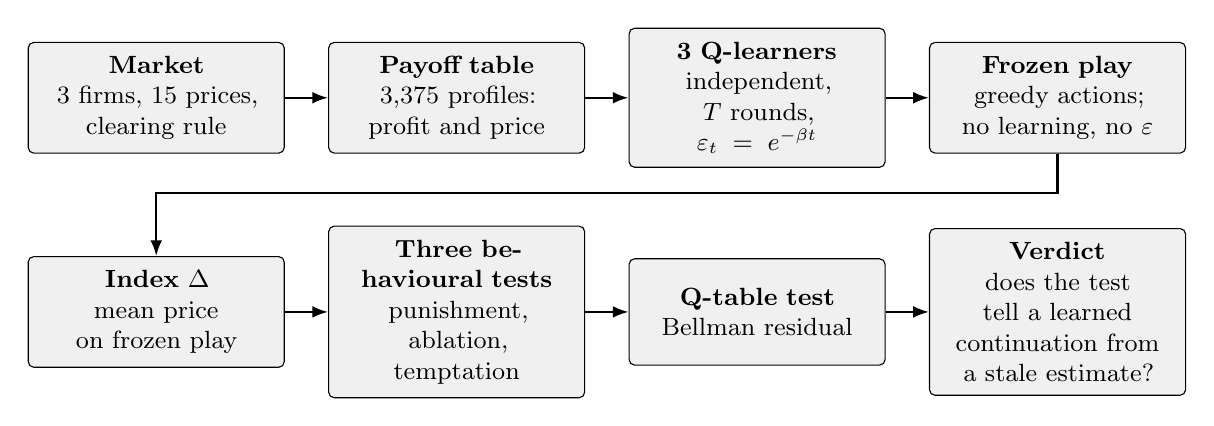
\begin{tikzpicture}[
  font=\small,
  box/.style={draw=black, fill=black!6, rounded corners=2pt, align=center,
              text width=2.9cm, inner sep=5pt, minimum height=1.35cm},
  arrow/.style={-{Latex[length=2mm]}, thick, draw=black},
  node distance=0.55cm and 0.55cm
]
\node[box] (market) {\textbf{Market}\\ 3 firms, 15 prices,\\ clearing rule};
\node[box, right=of market] (table) {\textbf{Payoff table}\\ 3,375 profiles:\\ profit and price};
\node[box, right=of table] (learners) {\textbf{3 Q-learners}\\ independent, $T$ rounds,\\ $\varepsilon_t = e^{-\beta t}$};
\node[box, right=of learners] (freeze) {\textbf{Frozen play}\\ greedy actions;\\ no learning, no $\varepsilon$};
\node[box, below=1.3cm of market] (delta) {\textbf{Index $\Dl$}\\ mean price\\ on frozen play};
\node[box, right=of delta] (behav) {\textbf{Three behavioural tests}\\ punishment, ablation,\\ temptation};
\node[box, right=of behav] (qtable) {\textbf{Q-table test}\\ Bellman residual};
\node[box, right=of qtable] (verdict) {\textbf{Verdict}\\ does the test tell a learned\\ continuation from a stale estimate?};
\draw[arrow] (market) -- (table);
\draw[arrow] (table) -- (learners);
\draw[arrow] (learners) -- (freeze);
\draw[arrow] (freeze.south) -- ++(0,-0.5) -| (delta.north);
\draw[arrow] (delta) -- (behav);
\draw[arrow] (behav) -- (qtable);
\draw[arrow] (qtable) -- (verdict);
\end{tikzpicture}
\caption{The pipeline. The payoff table is the clearing rule evaluated once on every bid profile; training, freezing, and every test read from it. $\Dl$, the punishment and temptation tests and the Bellman residual are computed on frozen greedy play, not on the training trace; the ablation retrains the learner and reads its $\Dl$ the same way; only the occupation measure of Section~\ref{sec:occupation} is measured while exploring. Of the four tests only the Q-table test tells a learned continuation from a stale estimate; the punishment test also differs across the two learners, but only because a one-state table has nothing to react to (Section~\ref{sec:discussion}).}
\label{fig:pipeline}
\end{figure}

\subsection{The auction}\label{sec:market}

Three symmetric firms, $i = 1, 2, 3$, each with 60~MW of capacity and a marginal cost of \eur{10}/MWh, bid into a single-node uniform-price auction with inelastic demand of 100~MW and a price cap of \eur{100}/MWh (Table~\ref{tab:market}). The setting follows \citet{seredynski2026} at single-node scale, with no network, no congestion and one demand level; the format is the multi-unit uniform-price auction of \citet{vonderfehr1993} and \citet{fabra2006}. Each round every firm submits one price from a grid of 15 rungs, $p_r = 10 + (r-1)\cdot 90/14$ for $r = 1, \dots, 15$, so one rung is \eur{6.43}.

\begin{table}[t]
\caption{Market parameters. Notes: the grid is $\mathrm{linspace}(10, 100)$ with 15 points; total capacity is 180~MW; any two firms cover demand ($120 \geq 100$), so no firm is pivotal.}
\label{tab:market}
\centering
\small
\begin{tabular}{llr}
\toprule
Parameter & Symbol & Value \\
\midrule
Firms & $n$ & 3 \\
Capacity per firm (MW) & $q_i$ & 60 \\
Marginal cost (\eur{}/MWh) & $c$ & 10 \\
Demand, inelastic (MW) & $D$ & 100 \\
Price cap (\eur{}/MWh) & $p_{\max}$ & 100 \\
Bid grid & $p_r$ & 15 rungs, 10 to 100 \\
Grid step (\eur{}/MWh) & & 6.43 \\
Competitive benchmark (\eur{}/MWh) & $p^{c}$ & 10 \\
Collusive benchmark (\eur{}/MWh) & $p^{m}$ & 100 \\
Collusion index & $\Dl$ & $(\bar p - 10)/90$ \\
\bottomrule
\end{tabular}
\end{table}

Bids are sorted in ascending order and dispatched in that order until 100~MW is covered. The clearing price $p$ is the bid of the last unit dispatched, every dispatched firm is paid $p$, and ties at the margin split the residual demand pro rata to capacity. Firm $i$ earns $(p - 10)\,x_i$ on its dispatched quantity $x_i \le q_i$.

The clearing rule has one property the rest of the paper relies on: the clearing price is always the second-lowest bid. The lowest bidder sells 60~MW, the second-lowest sells the remaining 40~MW, and the highest sells nothing unless tied. From any profile at which the two lowest bids are tied, including every symmetric profile, a lone one-rung undercut does not move the price; if the undercutter was one of the tied pair it becomes the lowest bidder and is paid the rivals' bid for its full 60~MW. When all three firms bid the cap, a lone one-rung undercut raises the undercutter's profit from \eur{3{,}000} to \eur{5{,}400} without moving the price, whereas when the two lowest bids differ an undercut that lands between them does move it, as at the most common memory-0 rest point, $(10, 100, 100)$, of Section~\ref{sec:results}, where a high bidder shaving one rung clears the market at \eur{93.57} and sells 40~MW. From a symmetric profile the price falls only when a second firm follows the first down. The punishment test below therefore judges reactions on the rivals' bids, not on the price.

The competitive benchmark is bidding at cost, $p^{c} = 10$; the collusive benchmark is the cap, $p^{m} = 100$, the joint-profit maximum under inelastic demand. Adapting the profit index of \citet{calvano2020} to prices, with cost rather than the one-shot Nash outcome as the zero, the collusion index is
\begin{equation}
\Dl = \frac{\bar p - 10}{100 - 10},
\end{equation}
where $\bar p$ is the mean clearing price on frozen play; $\Dl = 0$ at the competitive benchmark and $\Dl = 1$ at the cap. The pay-as-bid variant of Section~\ref{sec:phase1} keeps the dispatch rule but pays each dispatched firm its own bid; the reported price stays the marginal bid, so $\Dl$ remains comparable as an index of the marginal bid, though under pay-as-bid it is no longer the price every dispatched firm is paid.

Enumerating all 3,375 profiles gives seven pure Nash equilibria of the one-shot game, in three shapes (Table~\ref{tab:nash}). All three firms at cost is the non-pivotal equilibrium of \citet{vonderfehr1993}: when any two firms cover demand, competition drives the price to cost. In the other two, one firm bids cost and the two others tie one or two rungs above it; the tied firms gain nothing from the lower rungs open to them, and the low firm cannot gain by raising its bid. Profiles of this shape exist on any grid; their $\Dl$ is one or two rungs and shrinks with the rung, so they are a grid artefact in size rather than in kind. The consequence is that the competitive benchmark on this grid is a band, $\Dl \in [0, 0.14]$, rather than a point; every mean $\Dl$ reported later lies far above it; a few individual $\gamma = 0$ seeds do not (minimum 0.071, and the 5\% that end at a one-shot Nash profile).

\begin{table}[t]
\caption{Pure Nash equilibria of the one-shot game on the 15-rung grid. Notes: bids and price in \eur{}/MWh, profits in \eur{} per round, listed in the order of the bids shown; the second and third shapes each stand for three profiles (all permutations of the firms).}
\label{tab:nash}
\centering
\small
\begin{tabular}{llrrrr}
\toprule
Shape & Bids & Profiles & Price & Profits & $\Dl$ \\
\midrule
All at cost & (10, 10, 10) & 1 & 10.00 & (0, 0, 0) & 0.00 \\
One at cost, two tied one rung up & (10, 16.43, 16.43) & 3 & 16.43 & (386, 129, 129) & 0.07 \\
One at cost, two tied two rungs up & (10, 22.86, 22.86) & 3 & 22.86 & (771, 257, 257) & 0.14 \\
\bottomrule
\end{tabular}
\end{table}

\subsection{The learners}\label{sec:learners}

Each firm runs independent tabular Q-learning \citep{watkins1992}: one table per firm, no shared parameters, no communication, as in \citet{calvano2020}. Firm $i$ observes its own profit and the public record of last round's bids. The state $s_t$ is that record, the full bid profile of round $t-1$, so there are $15^3 = 3{,}375$ states and each table $Q_i(s, a)$ has $3{,}375 \times 15$ entries; we call this memory $m = 1$. The memory-0 variant ($m = 0$) has a single state, one row of 15 entries, so the learner cannot condition on anything. The action $a_{i,t}$ is a rung and the reward $\pi_{i,t}$ is the firm's own profit in round $t$. After each round every firm updates one entry,
\begin{equation}
Q_i(s_t, a_{i,t}) \leftarrow (1 - \alpha)\, Q_i(s_t, a_{i,t}) + \alpha \Big[ \pi_{i,t} + \gamma \max_{a'} Q_i(s_{t+1}, a') \Big],
\label{eq:qupdate}
\end{equation}
with $\alpha = 0.15$ and $\gamma = 0.95$. The $\gamma = 0$ variant keeps the state but values only the current round's profit.

Exploration is $\varepsilon$-greedy: in round $t$ each firm independently plays a uniformly random rung with probability $\varepsilon_t$ and otherwise $\arg\max_a Q_i(s_t, a)$, with
\begin{equation}
\varepsilon_t = e^{-\beta t}, \qquad \beta = 10^{-5},
\end{equation}
with its values at the horizons used tabulated in Appendix~\ref{app:params}. Exploratory bids enter the public record, and so the next state, like any other bid. Tables are initialised as in \citet{calvano2020}, $Q_0(s, a) = \mathbb{E}[\pi_i(a, a_{-i})]/(1 - \gamma)$ with rivals uniform on the grid; since the argmax breaks ties toward the lowest rung, an all-zero table would bias every unvisited state toward the lowest price.

The horizon is $T = 10^6$ rounds in the specification and $5 \times 10^6$ in the long runs, a horizon added after the 1M result was seen (Section~\ref{sec:design}); every run goes to its full horizon. A run is \emph{converged} if no firm's greedy action in any state changed during the last 100,000 rounds; the flag is recorded, not acted on. \emph{Frozen play} is greedy play with learning and exploration switched off. $\Dl$ is measured on frozen play: from the final state of training, play 1,000 greedy rounds, drop the first 100, and take the mean clearing price. The one exception, the time-average $\Dl$ of the exploring process in Section~\ref{sec:occupation}, is labelled as such.

\subsection{The indicators}\label{sec:indicators}

A supra-competitive $\Dl$ is an observation; tacit collusion is a claim about why the price sits there. We apply three behavioural indicators, the forced-deviation test of \citet{calvano2020}, a shortsightedness ablation that retrains the learner without a future or without a past, and an unclaimed-temptation test on the frozen cycle, and add a fourth test that reads the Q-table directly.

\paragraph{M3, punishment.} With learning frozen, the deviating firm is forced to bid \eur{10} for one round of greedy play, and the rivals' bids over the next 24 rounds are compared with a counterfactual path from the same state with no deviation, in two 12-round windows, rounds 1--12 and 13--24 (12 divides the cycle lengths 1--4 and 6; procedure and the 5- and 7-cycle caveat in Appendix~\ref{app:params}). \emph{Punish-forgive}: rivals bid at least half a rung (\eur{3.21}) below the counterfactual in rounds 1--12 and are back within half a rung in 13--24. \emph{Punish, no recovery}: below in both windows. \emph{No reaction}: the rivals' mean bid is not more than half a rung below the counterfactual in rounds 1--12. The three verdicts are exhaustive and exclusive; a deviator already bidding \eur{10} is flagged as a no-op, and each firm serves as deviator in turn. The verdict is read from the rivals' bids alone, not from the price or the deviator's own later bids, so a return to the old bid is not retaliation and the deviation round's profit does not enter it. That profit is never lower than before at the profiles the full learner converges to, and strictly higher unless the deviator was already the sole lowest bidder: it becomes (or remains) the lowest bidder and sells 60~MW at the lower of its rivals' bids. At a memory-0 rest point (low, high, high) a high bidder forced to \eur{10} drives the price down to the low bidder's bid and sells 60~MW at it; when the low bidder is at cost, as in the modal profile $(10, 100, 100)$ and in 36 of 100 long seeds, the price is \eur{10} and the deviator earns nothing that round.

\paragraph{M4, shortsightedness ablation.} The full learner is rerun with $\gamma = 0$ and, separately, with memory~0. If the high price were tacit collusion, which needs a future to care about and a past to condition on, both ablations should remove it. The criterion was fixed in advance: an ablated $\Dl$ has collapsed if it is below 0.25 and below half the full learner's $\Dl$. The indicator passes only if both collapse.

\paragraph{M5, unclaimed temptation.} Frozen play from the final state traces the cycle of greedy play; at 5M rounds this is the converged cycle, at 1M rounds, where no baseline seed met the convergence criterion, it is the cycle of the frozen but unconverged table. At every state on it, each firm's best one-shot deviation profit, rivals fixed at their greedy actions, is compared with its realised profit; among tied best deviations the smallest undercut is taken. The verdict is \emph{unclaimed temptation} if any gap is positive and \emph{static Nash} if every gap is zero. An unclaimed gap is necessary for the collusion reading, under which the profit is forgone because a reaction is anticipated; whether it is sufficient is what the memory-0 control tests.

\paragraph{Bellman residual.} The fourth test asks whether one fresh update of the unplayed deviation's value, using the continuation values already in the learner's table, would change its decision. For every temptation found by M5, with firm $i$ in state $s$ playing $a_i$ and best unplayed deviation $a_{\mathrm{dev}}$, let $s'$ be the state recorded if $a_{\mathrm{dev}}$ were played against the rivals' greedy actions $a_{-i}$ (the single state under memory~0). One application of equation~\eqref{eq:qupdate} would move the deviation's entry toward the target
\begin{equation}
y_i(s, a_{\mathrm{dev}}) = \pi_i(a_{\mathrm{dev}}, a_{-i}) + \gamma \max_{a'} Q_i(s', a'),
\qquad
\rho_i(s, a_{\mathrm{dev}}) = y_i(s, a_{\mathrm{dev}}) - Q_i(s, a_{\mathrm{dev}}),
\end{equation}
and $\rho_i$ is the Bellman residual on the deviation. On the played action the residual is near zero on every converged table (of order $10^{-11}$ for the full learner), as it must be at a rest point of the update; this serves as a check. The statistic reported is the share of temptations for which one backup already prefers the deviation, $y_i(s, a_{\mathrm{dev}}) > Q_i(s, a_i)$. We read a share of one as a deviation estimate that has not been refreshed since the rivals settled, since a single look would flip the decision; we read a share near zero as a learned continuation, since the state reached by deviating is worth less under the learner's own table. Both readings are interpretations of a one-step statistic, not properties it certifies. The test needs the Q-table, so it is a tool for simulations, not a screen for bid data; Section~\ref{sec:phase1} reports it and Section~\ref{sec:discussion} states its limits.

\section{Experimental design}\label{sec:design}

Table~\ref{tab:params} lists the parameters of the base design. Two pre-registered ablations change one learner parameter each ($\gamma = 0$ and memory~0, Section~\ref{sec:indicators}); the Phase~1 experiments each change one element of the design (the horizon following where the exploration schedule requires) and are specified in Section~\ref{sec:phase1}. The Market and Learner parameters, the 1M horizon and the convergence window come from the project specification; the seeds per cell, the frozen-play length, its burn-in and the CI rule are project choices; all were fixed before any result was seen and none was tuned. The one base parameter added after a result was seen is the 5M horizon (``Two horizons'' below). Apart from $\beta$ and the horizon no hyperparameter was varied in search of a result; the constant-$\varepsilon$ levels of Section~\ref{sec:occupation} and the two restart levels $\varepsilon_0$ of Section~\ref{sec:reinject} are the independent variables of those experiments, fixed with their predictions.

\begin{table}[htbp]
\centering
\caption{Parameters of the base design. Notes: the Market and Learner groups, the 1M horizon and the convergence window come from the specification; the seeds per cell, frozen-play length, burn-in and CI rule are design choices fixed before any result was seen; the 5M horizon was added after the 1M results (see ``Two horizons''); the punishment windows and threshold and the collapse criterion are discussed under ``What was fixed in advance''; ``rounds'' means auction rounds; SE is the standard error across seeds.}
\label{tab:params}
\begin{tabular}{llr}
\toprule
Group & Parameter & Value \\
\midrule
Market & Firms & 3 \\
 & Capacity per firm & 60 MW \\
 & Marginal cost & \eur{10}/MWh \\
 & Demand (inelastic) & 100 MW \\
 & Price cap & \eur{100}/MWh \\
 & Bid grid & 15 rungs, \eur{10} to \eur{100} \\
 & Grid rung & \eur{6.43} \\
Learner & Learning rate $\alpha$ & 0.15 \\
 & Discount $\gamma$ & 0.95 (ablation: 0) \\
 & Exploration decay $\beta$ & $10^{-5}$ (sweep: $10^{-6}$ to $10^{-4}$) \\
 & Memory $m$ & 1 (ablation and control: 0) \\
 & States, $m=1$ & 3,375 \\
 & Initial table $Q_0$ & $\mathbb{E}[\text{profit}(a,\ \text{rivals uniform})]/(1-\gamma)$ \\
Run & Horizon $T$ & 1M and 5M rounds \\
 & Convergence window & 100,000 rounds \\
 & Frozen play & 1,000 rounds \\
 & Frozen burn-in dropped & 100 rounds \\
 & Seeds per cell & 100 \\
 & CI rule & mean $\pm 1.96 \times$ SE \\
Punishment test & Settling rounds & 200 \\
 & Pre / post rounds & 6 / 24 \\
 & Judgement windows & 2 $\times$ 12 rounds \\
 & Reaction threshold & half a rung (\eur{3.21}) \\
Ablation & Collapse criterion & $\Dl < 0.25$ and $< \tfrac{1}{2}$ full learner \\
\bottomrule
\end{tabular}
\end{table}

\paragraph{What was fixed in advance, and what was not.}
``Pre-registered'' here means written down in the project's own documents before the corresponding runs; there is no public registry entry, and the record is a git history rather than a timestamped filing. Three levels should be distinguished, because they do not carry equal weight.

The specification, written before any code, fixes the market, the learners, every hyperparameter in the Market and Learner groups of Table~\ref{tab:params}, the 1M horizon, the four measurements, and acceptance rules stated in words: a meaningful fraction of seeds above $\Dl = 0.5$ for M2; prices that drop below the pre-deviation level and then recover for M3; $\Dl$ collapsing toward zero under both ablations for M4; at least one strictly profitable unplayed deviation for M5. None of these carries a number.

The numerical thresholds were therefore fixed one level down, in the implementation, and are present in the first committed version of the code, before any run reported here. They are the collapse rule for M4 ($\Dl < 0.25$ and below half the full learner's $\Dl$) and the whole operationalisation of M3: judging on the rivals' bids against a no-deviation counterfactual, in two 12-round windows, with a half-rung threshold. Two of these choices were informed by earlier runs and we flag them rather than claim more than the record supports. The 12-round window length is justified by the converged cycle lengths, which were known only after the first runs: it lets a cycle of period 1, 2, 3, 4 or 6 complete a whole number of times in each window, while periods 5 and 7, which occur in 9 of the 100 long-run seeds, are not covered and can be misread (Section~\ref{sec:discussion}); at 1M rounds, where periods run up to 56 and only 23 of 100 seeds have period four or less, the 12-seed verdicts of Table~\ref{tab:m3} are more exposed to this than the long-run ones. And the rival-bid criterion replaced an earlier price-based one after the price-based version was found to read a converged cycle's own price dip as punishment. Every M3 verdict reported here was computed with the final criterion, and no verdict computed under the earlier one is reported.

The Phase~1 experiments are not in the specification at all. They were designed after the results of Section~\ref{sec:results} were seen, and sequentially, each in response to the last. What was fixed in advance there is narrower: each experiment's prediction was written into the script before that experiment ran, and all five are reported with their outcomes, two of which failed outright, in Section~\ref{sec:phase1}.

\paragraph{Acceptance rules.}
No numerical acceptance threshold for M2 is on record: the specification asks for a meaningful fraction of seeds that converge to $\Dl > 0.5$. We report the share of seeds above $\Dl = 0.5$ and call M2 met only where every seed exceeds it, which is the case at 5M rounds (100\%, all converged) and not at 1M (12\%, none converged); readers who accept a lower threshold may read the 1M result differently. M3 is judged with firm~1 as the forced deviator, the code's default; the verdicts for firms~2 and~3 are reported in Appendix~\ref{app:extra}, and no rule for combining the three was fixed in advance. M4 is met only if both ablated learners collapse, $\Dl < 0.25$ and below half the full learner's $\Dl$. M5 is a necessary condition: the collusion reading requires an unclaimed gap, and the memory-0 control tests whether it is sufficient. The outcome is read as supporting tacit collusion only if M2, M3 (punish--forgive) and M4 are all met and M5 fires for the memory-1 learner but not for the control.

\paragraph{Seeds and confidence intervals.}
Every configuration is run on 100 independent seeds; where a table reports a subset (the seeds with $\Dl > 0.5$, labelled ``collusive'' in Section~\ref{sec:results}) it says so. A seed fixes the random draws of a run; the initial tables are deterministic. Means are reported with a 95\% confidence interval of mean $\pm 1.96$ times the standard error across seeds; medians, ranges and per-seed counts are reported with the price levels in Section~\ref{sec:results}. A 50-seed run of the whole study preceded the 100-seed run, on the first 50 of the same seeds; every $\Dl$ moved by at most 0.02 between the two, and no verdict changed.

\paragraph{Two horizons.}
At the specified $T = 1$M rounds the learners are almost greedy ($\varepsilon_t = 4.5 \times 10^{-5}$, Section~\ref{sec:learners}), yet $\Dl = 0.375$, no seed meets the convergence criterion and M2 is not met (Section~\ref{sec:results}). The 5M-round horizon is not in the specification: it was added after that result was seen and is not pre-registered, and every base configuration converges in every seed there. It is one of two cells chosen after seeing the quantity it reports; the other is the 30M-round $\varepsilon = 10^{-4}$ point of Table~\ref{tab:occupation}, added once the memory-1 occupation curve was seen still rising at $\varepsilon = 10^{-3}$ (Section~\ref{sec:occupation}). We report both horizons: M2 fails at 1M and is met at 5M, M4 and M5 give the same verdict at both, and M3 is judged on 12 seeds at 1M and on all 100 at 5M; the headline $\Dl = 0.621$ comes from the added one. Every run goes to its full horizon.

\paragraph{What is measured, and on what.}
$\Dl$ and all behavioural indicators are computed on frozen play as defined in Section~\ref{sec:indicators}: 1,000 greedy rounds from the final state, the first 100 dropped. Outside the constant-$\varepsilon$ experiment of Section~\ref{sec:occupation}, no reported $\Dl$ or verdict is computed on the training trace, because it mixes exploration draws with the learned policy in a share that changes with $t$; the training-trace prices in Figures~\ref{fig:trajectory} and~\ref{fig:trajectory5m} and the lowest 1,000-round mean of Table~\ref{tab:reinject} are descriptive only. Frozen play isolates the greedy policy from the final state; it visits only the cycle reachable from that state, and M5 and the Bellman residual are computed on that cycle alone. The punishment test adapts the one-round forced deviation of \citet{calvano2020}, with the verdict read on the rivals' bids against a no-deviation counterfactual because, from any profile at which the two lowest bids are tied, a lone undercut does not move the price (Section~\ref{sec:market}), so the price is an unreliable signal of a reaction.

\paragraph{The memory-0 control.}
The memory-0 learner sees one state, so it cannot condition on what rivals did last round and cannot carry a threat; on the working definition of Section~\ref{sec:related}, a firm holding back because it expects retaliation \citep{tirole1988,ivaldi2003}, whatever price it reaches is by construction not tacit collusion. In a Q-learner such a threat, if it exists, lives in the learned continuation values, and the control calibrates the indicators against that. An indicator that reads the same on both learners does not by itself distinguish a learned continuation from a stale estimate; and an indicator that separates them because a one-state table has nothing to react to shows that the memory-1 policy conditions on rivals' bids, which its state permits but does not guarantee, and not that the conditioning is a threat (Section~\ref{sec:discussion}).

\paragraph{Compute and reproducibility.}
The auction and learning loop are compiled with numba and run at about 0.4~s per 1M rounds per seed; the six base configurations at 100 seeds take about 9 minutes and the whole study about two hours sequentially on a laptop with no GPU. The code is the Python package \texttt{collusim} v0.1.0 with 31 tests (Appendix~\ref{app:repro}); every simulation number in this paper is taken from the stored \texttt{results/*.json} files, which the scripts described there produce, and the one-shot payoffs, Nash equilibria and deviation gains of Section~\ref{sec:market} are computed from the payoff table with the same package.

% 05_results.tex — owned by this file: sec:results, tab:m2, tab:m3, tab:m4, tab:m5,
% fig:trajectory, fig:trajectory5m, fig:punishment, fig:ablation.
% Every number here is taken from paper/FACTS.md.

\section{Results: prices and the three behavioural tests}\label{sec:results}

This section reports the four pre-registered measurements of Section~\ref{sec:design}: the price level (M2), the reaction to a forced undercut (M3), the shortsightedness ablation (M4) and the unclaimed-temptation test (M5). Every cell has 100 seeds. $\Dl$ is measured on frozen greedy play after training; confidence intervals are mean $\pm\,1.96$ standard errors across seeds; ``high-price seeds'' are seeds with $\Dl > 0.5$. The pay-as-bid runs belong to Section~\ref{sec:phase1}.

\subsection{M2: price levels}

Table~\ref{tab:m2} gives $\Dl$ for the full learner and the two ablated learners at both horizons.

\begin{table}[htbp]
\centering
\caption{M2: collusion index $\Dl$ on frozen greedy play, 100 seeds per row. Notes: CI is the 95\% interval across seeds; ``converged'' means no firm's greedy action changed in the last 100,000 training rounds; the ablated learners are defined in Section~\ref{sec:learners}.}
\label{tab:m2}
\small
\setlength{\tabcolsep}{4pt}
\begin{tabular}{@{}llrrrrrr@{}}
\toprule
Learner & $T$ & $\Dl$ mean & 95\% CI & Median & Min--max & Seeds $\Dl>0.5$ & Converged \\
\midrule
Full ($\gamma=0.95$, $m=1$) & 1M & 0.375 & 0.354--0.397 & 0.343 & 0.143--0.679 & 12\% & 0\% \\
Full ($\gamma=0.95$, $m=1$) & 5M & 0.621 & 0.612--0.630 & 0.625 & 0.518--0.714 & 100\% & 100\% \\
$\gamma=0$, $m=1$ & 1M & 0.373 & 0.353--0.393 & 0.386 & 0.071--0.619 & 5\% & 0\% \\
$\gamma=0$, $m=1$ & 5M & 0.370 & 0.350--0.390 & 0.386 & 0.071--0.619 & 4\% & 100\% \\
$\gamma=0.95$, $m=0$ & 1M & 0.943 & 0.931--0.955 & 0.929 & 0.714--1.000 & 100\% & 79\% \\
$\gamma=0.95$, $m=0$ & 5M & 0.943 & 0.931--0.954 & 0.929 & 0.714--1.000 & 100\% & 100\% \\
\bottomrule
\end{tabular}
\end{table}

\paragraph{At the pre-registered horizon nothing has converged.}
At the specified horizon the full learner reaches $\Dl = 0.375$ (CI 0.354--0.397), a mean frozen clearing price of \eur{43.8}/MWh, and no seed has converged. The spread is wide: 1 seed below 0.2, 85 between 0.2 and 0.5, and 14 at or above 0.5 (12 strictly above).
% TODO-FACT: FACTS.md gives "14 in [0.5,0.7)" and "12% with Δ>0.5" separately; the 2 seeds at exactly Δ = 0.5 (price €55.00) should be entered in FACTS.md §3.
Figure~\ref{fig:trajectory} shows the process still moving. The mean price falls to about \eur{40} early in the run, while $\varepsilon_t$ is still large, and then drifts up; a few seeds jump to a higher band before the horizon. We read the early fall as the learners finding the undercut, but this section does not test that reading.
% TODO-FACT: round at which the mean price first reaches €40 and the timing of the late jumps are not in FACTS.md.

\begin{figure}[htbp]
\centering

\includegraphics[width=\textwidth]{figures/price_trajectory.png}
\caption{Mean clearing price per 1,000 rounds during training, full learner, 1M rounds. Thin lines are the 100 seeds; the thick line is their mean. Dashed lines mark the competitive (\eur{10}) and collusive (\eur{100}) benchmarks.}
% TODO-FACT: block length of the trajectory figures (collusim.agents.BLOCK) is not in FACTS.md; enter the figure script's settings there.
\label{fig:trajectory}
\end{figure}

Five million rounds finish the process (Figure~\ref{fig:trajectory5m}). Seeds leave the \eur{40} band one at a time, jump to a mean price between \eur{60} and \eur{72}, and never move again. Every seed converges; the round of the last change in any firm's greedy action has median 1.63M (range 1.20M--2.88M).
% TODO-FACT: confirm this is how the convergence round is defined in results/*.json.
All land in a narrow band: $\Dl = 0.621$ (CI 0.612--0.630), 99 seeds in $[0.5, 0.7)$ and one above, mean frozen price \eur{65.9}/MWh. The acceptance criterion for M2 fails at the pre-registered 1M horizon and is met at 5M, a horizon added after the 1M result was seen and not itself pre-registered (Section~\ref{sec:design}). The M2 criterion was written as `a meaningful fraction of seeds above $\Dl = 0.5$' without a number; we read 12\% at 1M as failing it and 100\% at 5M as meeting it, and a reader who counts 12\% as meaningful should treat M2 as met at both horizons.
% TODO-FACT: the pre-registered wording of the M2 rule.
The ablated learners converge sooner: median 1.26M rounds (1.14M--1.45M) for $\gamma = 0$ and 0.83M (0.72M--0.99M) for memory 0.

\begin{figure}[htbp]
\centering
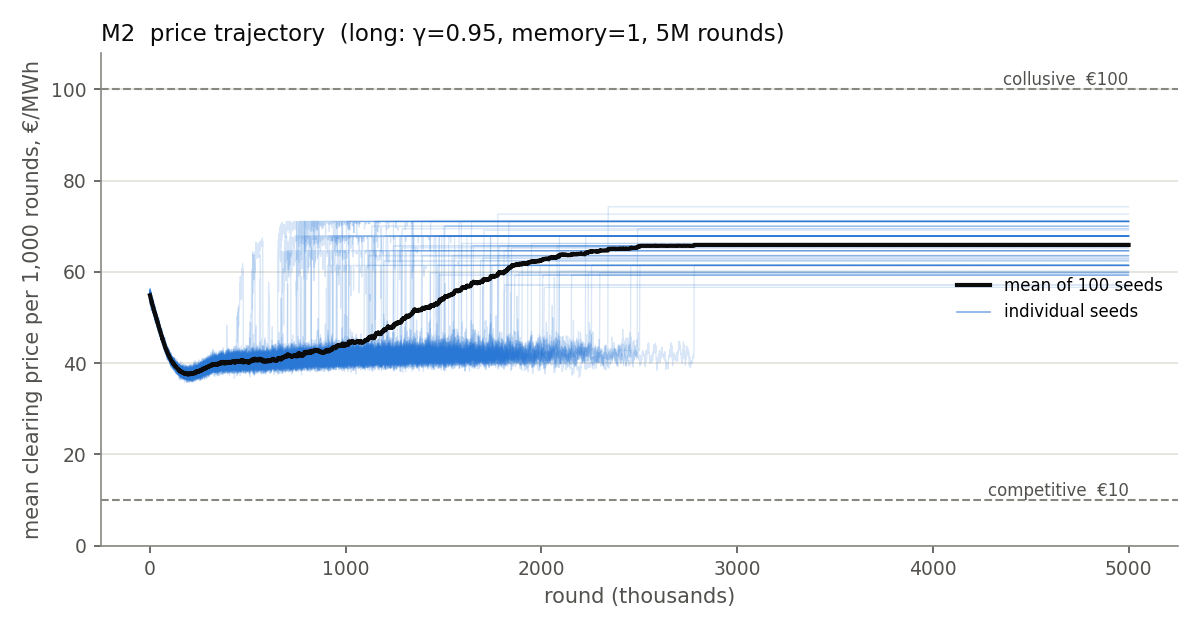
\includegraphics[width=\textwidth]{figures/price_trajectory_long.png}
\caption{As Figure~\ref{fig:trajectory}, for 5M rounds. Seeds jump one at a time from the \eur{40} band to \eur{60}--\eur{72} between roughly 1.2M and 2.9M rounds and then stay there.}
\label{fig:trajectory5m}
\end{figure}

\paragraph{What the converged policies do.}
The converged full learners do not sit at a constant high price. Reading the frozen state sequence, 86 of 100 seeds play a cycle of period four or less (period 1: 3 seeds; 2: 35; 3: 21; 4: 27); the rest run 5-, 6- or 7-cycles (7, 5 and 2 seeds). The 35 two-cycles alternate a near-symmetric high profile, bids \eur{94}--\eur{100} with mean high price \eur{96.5}, and a near-symmetric low profile, bids \eur{36}--\eur{42} with mean low price \eur{41.0}. Bid profiles are quoted rounded to the euro; the rungs are $10, 16.43, \dots, 93.57, 100$ (Section~\ref{sec:market}). One example is a seed that bids $(100, 94, 100)$ in round $t$, clearing at \eur{100}, then $(36, 42, 36)$ in round $t+1$, clearing at \eur{36}, and repeats. The most common last-round profiles are $(100,100,100)$ in 13 seeds and $(94,94,94)$ and $(36,42,42)$ in 6 each. At 1M rounds, before convergence, periods range from 1 to 56 and only 23 seeds have period four or less.

The $\gamma = 0$ learner converges to long, irregular cycles (20 of 100 seeds with period four or less, periods up to 25) whose most common last-round profiles have one firm at cost: $(10,16,16)$ in 15 seeds, $(10,36,36)$ and $(10,42,42)$ in 10 each.

The memory-0 learner converges at 5M rounds, in all 100 seeds, to a fixed point of the form (low, high, high): one firm bids low and the other two tie high. The low bidder sits at \eur{10} in 36 seeds, \eur{16.43} in 31, \eur{22.86} in 18, \eur{29.29} in 11, and \eur{42.14} or \eur{67.86} in 2 each; the high pair sits at the cap in 43 seeds, at \eur{93.57} in 36, at \eur{87.14} in 20 and at \eur{74.29} in 1. The most common profile, $(10,100,100)$, appears in 21 seeds. Because the clearing price is the second-lowest bid, it equals the high bid; the low bidder sells 60 MW at that price and earns the most, and each high bidder sells 20 MW. The mean frozen price is \eur{94.9}/MWh, $\Dl = 0.943$. None of these fixed points is a one-shot Nash equilibrium of Table~\ref{tab:nash}: at $(22.86, 100, 100)$, for example, each high bidder earns \eur{1{,}800} per round and could earn \eur{3{,}343} by bidding \eur{93.57}. Section~\ref{sec:phase1} returns to this.

\subsection{M3: punishment}

The punishment test adapts the impulse-response design of \citet{calvano2020}. With learning frozen, greedy play settles for 200 rounds, six pre-deviation rounds are recorded, one firm is forced to bid \eur{10} for a single round, and 24 rounds of greedy play follow. The verdict is read from the rivals' bids against a counterfactual path with no deviation, so that a converged cycle is not mistaken for a reaction, in two 12-round windows (12 divides the cycle lengths 1--4 and 6). ``Punish-forgive'': rivals at least half a rung (\eur{3.21}) below the counterfactual in rounds 1--12 and back within half a rung in rounds 13--24. ``Punish, no recovery'': below in both windows. ``No reaction'': rivals' bids do not move. Table~\ref{tab:m3} reports the verdicts with firm 1 as the deviator.

\begin{table}[htbp]
\centering
\caption{M3: verdicts of the punishment test, deviator firm 1. Notes: ``no-op'' counts seeds in which the deviator was already bidding \eur{10}, so the forced deviation changed nothing; those seeds are still judged. A no-op is ``no reaction'' by construction, since the forced bid equals the counterfactual; the no-op share is therefore part of the no-reaction share. Seed counts are in parentheses for the rows with fewer than 100 seeds. The last column counts seeds with a punish-forgive verdict for at least one of the three possible deviators.}
% TODO-FACT: the parenthesised counts are percentage × seeds judged (e.g. 33% of 12 = 4); confirm against results/indicators_*.json and enter the counts in FACTS.md §4.
\label{tab:m3}
\footnotesize
\setlength{\tabcolsep}{3pt}
\begin{tabular}{@{}llrrrrrr@{}}
\toprule
 & & & Punish-- & Punish, & No & & Forgive, \\
Learner & $T$ & Seeds & forgive & no recovery & reaction & No-op & $\geq 1$ deviator \\
\midrule
Full ($\gamma=0.95$, $m=1$) & 1M & 12 ($\Dl>0.5$) & 33\% (4) & 50\% (6) & 17\% (2) & 8\% (1) & 67\% (8) \\
Full ($\gamma=0.95$, $m=1$) & 5M & 100 (all) & 21\% & 70\% & 9\% & 2\% & 47\% \\
$\gamma=0$, $m=1$ & 1M & 5 ($\Dl>0.5$) & 0\% (0) & 20\% (1) & 80\% (4) & 40\% (2) & 40\% (2) \\
$\gamma=0$, $m=1$ & 5M & 4 ($\Dl>0.5$) & 25\% (1) & 25\% (1) & 50\% (2) & 25\% (1) & 50\% (2) \\
$\gamma=0.95$, $m=0$ & 1M / 5M & 100 (all) & 0\% & 0\% & 100\% & 10\% / 11\% & 0\% \\
\bottomrule
\end{tabular}
\end{table}

\begin{figure}[htbp]
\centering

\includegraphics[width=\textwidth]{figures/punishment_long.png}
\caption{M3 in the 5M full-learner runs. Left: bids and clearing price around the forced deviation for the seed with the highest $\Dl$ (the figure's agents 0, 1, 2 are firms 1, 2, 3). Right: mean clearing price across all 100 seeds, with the no-deviation counterfactual dotted.}
% TODO-FACT: which seed the left panel shows is not in FACTS.md; enter the figure script's seed selection there. When figures/punishment_long.png is regenerated, relabel its legend "firm 1/2/3" and delete the parenthetical (appendix.tex carries the canonical 0,1,2 mapping).
\label{fig:punishment}
\end{figure}

\paragraph{Reading.}
In the converged 5M runs a deviation is answered in 91\% of seeds. Over all 100 seeds the rivals' bids over rounds 1--12 average \eur{16.7} below the counterfactual, and the mean clearing price falls from \eur{66.0} to \eur{45.1} against a counterfactual of \eur{65.9}. The second window splits the 91\%. In 21\% the rivals are back by rounds 13--24: their drop shrinks from \eur{10.9} to \eur{0.2} and the price in that window is \eur{63.2} against \eur{65.4}. That is the punish-then-forgive pattern. In 70\% the rivals drop \eur{20.5} and are still \eur{19.1} below in the second window; the price stays at \eur{41.8} and then \eur{43.8} against \eur{66.2}. The test does not say whether this is a learned response to the deviation or the absence of any learned route back to the cycle; Section~\ref{sec:residual} bears on that question. In 9\% the rivals never move. Nine of the 100 long-run seeds play 5- or 7-cycles, which the 12-round windows do not cover; their verdicts can be misread, and the forgive/no-recovery split should be read with that in mind (Section~\ref{sec:discussion}).

Changing the deviator gives the same split in aggregate (firm 2: 20 forgive, 69 no recovery, 11 none; firm 3: 17, 73, 10), but the verdict for a given seed changes with the deviator in 61 of 100 seeds. The verdict is therefore a property of the seed and the deviator together, not of the seed alone. Part of this is mechanical: at the asymmetric profiles many seeds converge to, forcing a different firm to \eur{10} is a different deviation. The memory-0 control behaves as it must: with a single state there is nothing to react to, and 100\% of seeds show no reaction. The test therefore reads differently on the two learners, but for a reason that has nothing to do with strategy: a one-state table cannot react to anything, so the test detects the state definition, not a learned continuation (Section~\ref{sec:discussion}). The memory-1 learner passes its weak form (rivals react) in 91\% of seeds and its full form (react, then forgive) in 21\%.

From a profile at which the two lowest bids are tied, which includes the symmetric profiles the full learner converges to, the one-round deviation is profitable for the deviator and leaves the clearing price unchanged, because the price is the second-lowest bid; from an asymmetric profile, such as the memory-0 rest point, it can move the price and need not be profitable (Section~\ref{sec:market}). Section~\ref{sec:phase1} uses this.

\subsection{M4: shortsightedness ablation}

The ablation asks whether the high price needs memory of the past or a value on the future. The collapse criterion was fixed in advance: an ablated learner has collapsed if its $\Dl$ is below 0.25 and below half the full learner's $\Dl$. Table~\ref{tab:m4} and Figure~\ref{fig:ablation} give the outcome.

\begin{table}[htbp]
\centering
\caption{M4: collusion index of the full learner and the two ablated learners, with the pre-registered verdict. Notes: collapse requires $\Dl < 0.25$ and $\Dl$ below half the full learner's value.}
\label{tab:m4}
\begin{tabular}{lrrrl}
\toprule
$T$ & Full learner & $\gamma=0$ & Memory 0 & Verdict \\
\midrule
1M & 0.375 & 0.373 (not collapsed) & 0.943 (not collapsed) & fail \\
5M & 0.621 & 0.370 (not collapsed) & 0.943 (not collapsed) & fail \\
\bottomrule
\end{tabular}
\end{table}

\begin{figure}[htbp]
\centering

\includegraphics[width=\textwidth]{figures/ablation_bars.png}
\caption{M4 ablation at 1M rounds (left) and 5M rounds (right). Bars are the mean $\Dl$ across 100 seeds, whiskers the 95\% CI, dots the individual seeds.}
\label{fig:ablation}
\end{figure}

The test fails at both horizons. Removing the future ($\gamma = 0$) leaves $\Dl$ at 0.373 at 1M and 0.370 at 5M. At the specified horizon, where neither learner has converged, this is statistically indistinguishable from the full learner (0.375 against 0.373). At 5M the myopic learner does sit lower, 0.370 against 0.621: setting $\gamma = 0$ removes about 40\% of the converged price premium, not all of it, and 0.370 is far from collapse. Removing the past does the opposite of what the criterion anticipates: the memory-0 price rises to $\Dl = 0.943$ at both horizons. By the specification's own rule the M2 result cannot be attributed to tacit collusion on this evidence. The two ablated learners reach their prices by different routes, long irregular cycles in one case and an asymmetric fixed point in the other, but the ablation compares only $\Dl$ and cannot tell them apart.

\subsection{M5: unclaimed temptation}

At every state on the cycle of frozen play (the converged cycle at 5M; at 1M, the cycle of the frozen but unconverged table, Section~\ref{sec:indicators}), for each firm, the test computes the best one-shot deviation profit minus the realised profit, rivals held fixed. The verdict is ``unclaimed temptation'' if any gap is positive and ``static Nash'' if all gaps are zero.

\begin{table}[htbp]
\centering
\caption{M5: seeds with a profitable, unplayed one-shot deviation on the cycle of frozen play, and the mean best gap per round over seeds with $\Dl > 0.5$.}
\label{tab:m5}
\small
\begin{tabular}{@{}lrr@{}}
\toprule
Configuration & Seeds with unclaimed temptation & Mean best gap (\eur{}/round) \\
\midrule
Full ($\gamma=0.95$, $m=1$), 1M, $\Dl>0.5$ & 100\% (100\% of all seeds) & 2,475 \\
Full ($\gamma=0.95$, $m=1$), 5M & 100\% & 2,226 \\
$\gamma=0$, 1M / 5M & 100\% of $\Dl>0.5$ (95\% of all seeds) & 1,209 / 1,221 \\
Memory 0, 1M / 5M (control) & 100\% & 1,444 / 1,448 \\
\bottomrule
\end{tabular}
\end{table}

The temptation is large and, outside the 5\% of $\gamma = 0$ seeds that end at one-shot Nash profiles, present in every seed (Table~\ref{tab:m5}). At the all-cap profile each firm earns \eur{3{,}000} per round and could earn \eur{5{,}400} by shaving one rung off its bid: the price would not move and the firm would sell its full 60 MW. Nobody does. Read on its own, and only for the memory-1 learner, this is what the literature treats as the fingerprint of anticipated retaliation, and M3 would appear to agree. But the memory-0 control leaves the same kind of money on the table in 100\% of seeds, a mean gap of \eur{1{,}444} to \eur{1{,}448} per round, while being structurally incapable of anticipating anything. The 5\% of $\gamma = 0$ seeds without temptation sit at one-shot Nash profiles such as $(10,16,16)$. In this market the fingerprint is produced by a learner with no memory as readily as by one with memory, so on its own it is not discriminating.

\paragraph{Summary of verdicts.}
M2 fails at the pre-registered horizon and is met only at the 5M horizon added afterwards. M3 is partial: rivals react to a forced undercut in 91\% of converged seeds and forgive within 24 rounds in 21\%, and the memory-0 control shows no reaction in any seed. M4 fails at both horizons: neither ablation collapses the price, and the memory-0 learner prices higher than the full learner. The M5 fingerprint is present in 100\% of seeds, but equally in the memory-0 control. The learners converge to supra-competitive prices under these parameters, and the standard indicators do not support calling the outcome tacit collusion; none of the three behavioural tests separates a learner that has learned a continuation from one that carries a stale estimate; M3 reads differently on the two learners only because a one-state table has nothing to react to. Section~\ref{sec:phase1} asks what does, and Section~\ref{sec:discussion} collects the verdicts in Table~\ref{tab:indicators-summary}.

% 06_phase1.tex — owned by the phase1 writer. Numbers: paper/FACTS.md §1, §3, §7, §8 only.
\section{Strategy or frozen learning?}\label{sec:phase1}

Section~\ref{sec:results} ends with a puzzle. The memory-0 learner cannot condition on the past, so it cannot punish, yet it freezes at $\Dl = 0.943$, above the full learner's $0.621$, and the temptation test of Section~\ref{sec:indicators} fires for it all the same, while the ablation reads it as the higher-priced learner. The natural guess is that its high price is an accident of the exploration schedule: $\varepsilon_t$ died before an undercutting race could finish, and the tables froze with stale estimates of what an undercut is worth. This section tests that guess. Five experiments were designed, and their predictions written down, before any of them ran. Each cell uses 100 seeds and the hyperparameters of Section~\ref{sec:design}; each experiment changes one element of the design and, where the change forces it, the horizon or the quantity measured, as stated in its subsection. Table~\ref{tab:predictions} lists the predictions and the outcomes. Two of the five failed outright, two held only in part, and one held with a caveat (Table~\ref{tab:predictions}). The failures are the useful part: a ten-fold longer decay and a change to pay-as-bid do not remove the memory-0 price, which rules out the two readings we tested, a race cut short by the schedule and an artefact of the uniform-price rule in particular. The tables are stale (Section~\ref{sec:residual}), but the staleness is reproduced rather than accidental. Section~\ref{sec:occupation} offers a reading of why; it is a verbal argument, not a result.

\begin{table}[htbp]
\centering
\caption{Pre-registered predictions and outcomes.}
\label{tab:predictions}
\small
\begin{tabular}{@{}clp{5.6cm}p{4.6cm}@{}}
\toprule
\# & Experiment & Prediction & Held? \\
\midrule
1 & $\beta$ sweep (slower decay) & memory-0 $\Dl$ falls toward 0; memory-1 holds & no \\
2 & $\varepsilon$ re-injection & memory-1 re-converges to the same $\Dl$; memory-0 collapses & half: memory-1 yes; memory-0 also re-converges \\
3 & Bellman residual & memory-0 large (stale); memory-1 small (learned) & yes, with a twist: both stale, consequence differs \\
4 & pay-as-bid & (low, high, high) rest point vanishes; memory-0 $\Dl$ falls a lot & no: $\Dl$ falls 0.10, rest point moves, freeze stays \\
5 & constant-$\varepsilon$ occupation & frozen $\Dl = \lim_{\varepsilon\to 0}$ of the time-average $\Dl$ & memory-0 within 0.01; memory-1 within about 0.02 at one point, from above, and needing about 30$\times$ less noise \\
\bottomrule
\end{tabular}
\par\smallskip
\footnotesize Notes: predictions were fixed before the runs; 100 seeds per cell. Two of the five failed outright, two held only in part, and one held with a caveat.
\end{table}

\subsection{Slower exploration decay}\label{sec:beta}

If the memory-0 freeze is a race cut short, a longer race should finish it. The sweep varies $\beta$ in $\varepsilon_t = e^{-\beta t}$ over two orders of magnitude and sets the horizon to $10/\beta$ plus a 4M-round tail, so every cell reaches $\varepsilon = e^{-10}$ and then gets the same greedy tail. At $\beta = 10^{-6}$ the learners get ten times the exploratory rounds of the specification.

\begin{table}[htbp]
\centering
\caption{Frozen $\Dl$ against the exploration decay rate $\beta$.}
\label{tab:sweep}
\small
\begin{tabular}{@{}lrrrr@{}}
\toprule
$\beta$ & Rounds & Memory 0: $\Dl$ (95\% CI) & Memory 1: $\Dl$ (95\% CI) & Memory 1 converged \\
\midrule
$10^{-6}$ & 14M & 0.949 (0.936--0.962) & 0.721 (0.695--0.746) & 88\% \\
$3\times 10^{-6}$ & 7.3M & 0.940 (0.928--0.952) & 0.636 (0.623--0.649) & 100\% \\
$10^{-5}$ (spec) & 5M & 0.943 (0.931--0.954) & 0.621 (0.612--0.630) & 100\% \\
$3\times 10^{-5}$ & 4.3M & 0.957 (0.946--0.968) & 0.618 (0.610--0.626) & 100\% \\
$10^{-4}$ & 4.1M & 0.949 (0.938--0.961) & 0.593 (0.583--0.603) & 100\% \\
\bottomrule
\end{tabular}
\par\smallskip
\footnotesize Notes: horizon $= 10/\beta + 4$M rounds; 100 seeds per cell; memory-0 converged in 100\% of seeds in every cell.
\end{table}

Table~\ref{tab:sweep} rejects the prediction. Memory-0 is flat between 0.940 and 0.957 across the whole range, with overlapping confidence intervals, and it converges in every seed of every cell. A ten-fold longer race did not finish. Memory-1 does not hold either, so the second half of the prediction also fails: slower decay gives higher frozen prices, from 0.593 at $\beta = 10^{-4}$ to 0.721 at $\beta = 10^{-6}$, where 12\% of seeds had not met the convergence criterion by 14M rounds. Within the range tested, the length of a decaying exploration schedule does not change where the memory-0 learner freezes, and for the memory-1 learner slower decay is associated with a higher frozen price.

\subsection{Re-injecting exploration}\label{sec:reinject}

The second test starts from the converged 5M tables and restarts training with $\varepsilon_t = \varepsilon_0 e^{-\beta t}$, $\beta = 10^{-5}$, for 2M rounds, then freezes and measures $\Dl$ again. A learned equilibrium should re-converge to the same price. A stale-table accident should not survive $\varepsilon_0 = 0.5$, which makes half of all early actions random.

\begin{table}[htbp]
\centering
\caption{Re-injecting exploration into converged tables.}
\label{tab:reinject}
\footnotesize
\setlength{\tabcolsep}{4pt}
\begin{tabular}{@{}lrrrrr@{}}
\toprule
 & & $\Dl$ & Seeds & Lowest 1k-round & Low bidder \\
Source & $\varepsilon_0$ & before $\to$ after & dropping $>0.1$ & mean price & changed \\
\midrule
memory 1 & 0.05 & 0.621 $\to$ 0.622 & 4\% & \eur{38} & --- \\
memory 1 & 0.5 & 0.621 $\to$ 0.621 & 5\% & \eur{38} & --- \\
memory 0 & 0.05 & 0.943 $\to$ 0.945 & 11\% & \eur{37} & 71\% \\
memory 0 & 0.5 & 0.943 $\to$ 0.952 & 10\% & \eur{37} & 70\% \\
\bottomrule
\end{tabular}
\par\smallskip
\footnotesize Notes: 100 converged 5M tables per row; restart with $\varepsilon_t = \varepsilon_0 e^{-\beta t}$, $\beta = 10^{-5}$, 2M rounds, then frozen play. ``Low bidder changed'' is the share of memory-0 seeds in which a different firm holds the low bid after the restart.
\end{table}

Table~\ref{tab:reinject} shows that the mean frozen $\Dl$ of both learners returns to its pre-restart value. At $\varepsilon_0 = 0.5$ the memory-0 tables are scrambled: the lowest 1,000-round mean price during the run is \eur{37}, and in 70\% of seeds a different firm ends as the low bidder. The milder restart at $\varepsilon_0 = 0.05$ disrupts the tables just as much (lowest price \eur{37}, low bidder changed in 71\% of seeds), so the return does not depend on the size of the restart. The process nevertheless returns to a mean $\Dl$ of 0.952, with only 10\% of seeds dropping by more than 0.1, and all 100 seeds end again at a profile of the same (low, high, high) shape.
The estimates left behind are stale (Section~\ref{sec:residual}), but the restart reproduces the same kind of stale configuration with the roles reassigned, so the staleness is not an accident of one schedule; whatever produces it operates again whenever exploration fades. Section~\ref{sec:occupation} offers a reading. The memory-1 learner also re-converges, to 0.621 or 0.622, with 4--5\% of seeds dropping. Both learners re-converge, so robustness to a restart does not separate them.

\subsection{The Bellman residual on the temptation action}\label{sec:residual}

Section~\ref{sec:results} showed that the converged cycles carry an unplayed profitable deviation in every full-learner and memory-0 seed. The question is what the table says about it. For every temptation on the converged cycle (firm $i$, state $s$, played action $a_i$, best unplayed deviation $a_{\mathrm{dev}}$) we compute the one-step target $\text{profit}(a_{\mathrm{dev}}, \text{rivals at their greedy actions}) + \gamma \max_a Q_i(s', a)$ and the residual $\text{target} - Q_i(s, a_{\mathrm{dev}})$, and the same for the played action. A residual near zero means the stored value of the deviation agrees with a one-step backup under the learner's own table; if the learner still declines it, the table values the state reached by deviating poorly, a continuation that may itself be stale (Section~\ref{sec:discussion}). A large residual is what one expects if $a_{\mathrm{dev}}$ has rarely or never been played since the rivals settled, so that its estimate dates from the exploration era. The share reported in Table~\ref{tab:residual} is the fraction of temptations for which the one-step target of the unplayed deviation, computed with the current table, exceeds the stored value of the played action, so that a refreshed estimate of the deviation would rank it above the played action.

\begin{table}[htbp]
\centering
\caption{Bellman residual on the temptation action, converged 5M tables.}
\label{tab:residual}
\footnotesize
\setlength{\tabcolsep}{4pt}
\begin{tabular}{@{}lrrrrr@{}}
\toprule
 & Residual, & Residual on $a_{\mathrm{dev}}$ & Share: one backup & Seeds at & Seeds with \\
Configuration & played & (95\% CI) & prefers $a_{\mathrm{dev}}$ & 0\% / 100\% & $\geq 1$ temptation \\
\midrule
Full (memory 1, $\gamma = 0.95$) & $\approx 0$ & \eur{\num{2708}} (\num{2521}--\num{2894}) & 31\% & 12 / 0 & 100 \\
$\gamma = 0$, memory 1 & $\approx 0$ & \eur{865} (824--907) & 100\% & 0 / 95 & 95 \\
Memory 0, $\gamma = 0.95$ & $\approx 0$ & \eur{\num{6656}} (\num{6093}--\num{7218}) & 100\% & 0 / 100 & 100 \\
\bottomrule
\end{tabular}
\par\smallskip
\footnotesize Notes: residual on the played action is of order $10^{-11}$ for the full learner. The five $\gamma = 0$ seeds without a temptation sit at one-shot Nash profiles and are not counted.
\end{table}

Played actions are Bellman-consistent everywhere, as they must be at a rest point of the update. The deviation estimates are non-zero-residual in every configuration, including the full learner, whose residual on $a_{\mathrm{dev}}$ is \eur{\num{2708}} (a difference of discounted values, so not directly comparable with the \eur{865} of the undiscounted $\gamma = 0$ table). The prediction that the memory-1 residual would be small therefore failed in its literal form. For $\gamma = 0$ and memory 0 a refreshed estimate of the deviation would flip the decision in 100\% of temptations, in every seed: the learner sits on money it has not looked at. For the full learner a refreshed estimate of the deviation would flip the decision in 31\% of temptations. In the other 69\% the value the learner's own table assigns to the state reached by deviating is low enough that a refreshed estimate would leave the deviation unattractive. Under the table's own valuation that is a learned continuation, the thing tacit collusion consists of; the valuation is a one-step backup whose continuation term may itself be stale (Section~\ref{sec:discussion}), and whether it deserves the name is not settled here.

The per-seed distribution is what makes this the discriminating test. Among the 100 full-learner seeds, 12 have a share of exactly 0\%, 71 lie in $(0, 50\%]$, 17 lie in $(50\%, 100\%)$, and none is at 100\%; the highest single seed is 80\%. Every memory-0 seed and every $\gamma = 0$ seed is at exactly 100\%. The two distributions do not overlap. Of the behavioural battery only M3 separates the two learners, and it does so because a one-state table cannot react (Section~\ref{sec:results}); the residual share separates them on what their tables value. The price of the test is that it reads the Q-table. It is a tool for simulated learners, not a screen for real bid data.

\subsection{Pay-as-bid}\label{sec:payasbid}

Under uniform pricing the profile (low, high, high) is a natural rest point for the memory-0 learner: the low bidder sells 60 MW at the high price and has no reason to move, and each high bidder can only discover the gain from a one-rung cut through an exploratory draw. If dispatched firms are paid their own bids instead, the low bidder is no longer paid the high price and should want to move up, so the rest point should vanish and $\Dl$ should fall sharply. The reported price stays the marginal bid, so $\Dl$ is comparable.

\begin{table}[htbp]
\centering
\caption{Pay-as-bid: frozen $\Dl$ and the most common frozen profiles, 5M rounds.}
\label{tab:payasbid}
\small
\begin{tabular}{@{}lrl@{}}
\toprule
Configuration & $\Dl$ (95\% CI) & Most common frozen profiles (seeds) \\
\midrule
memory 0, pay-as-bid & 0.845 (0.819--0.871) & (68,68,68) 16; (94,94,94) 12; (81,81,81) 9; (87,87,87) 8 \\
memory 1, pay-as-bid & 0.689 (0.677--0.701) & (55,55,55) 13; (49,49,55) 9; (61,61,61) 8; (49,49,49) 8 \\
\bottomrule
\end{tabular}
\par\smallskip
\footnotesize Notes: 100 seeds per row, converged 100\%. Profiles are the last-round bids in \eur{}/MWh, rounded; a symmetric tie splits the 100 MW three ways at each firm's own bid.
\end{table}

The rest point did vanish. Table~\ref{tab:payasbid} shows memory-0 freezing at symmetric ties, each firm selling a third of demand at its own bid, rather than at (low, high, high). But it freezes all the same, at $\Dl = 0.845$ against 0.943 under uniform pricing, a fall of 0.10. At every one of those ties each firm could gain by shaving one rung: from \eur{\num{1929}} to \eur{\num{3086}} per round at the tie at 67.86 (a gain of \eur{\num{1157}}), and from \eur{\num{2786}} to \eur{\num{4629}} at 93.57 (a gain of \eur{\num{1843}}), with the ties at 80.71 and 87.14 in between. The auction rule changes where the process stops, not whether it stops. The memory-1 learner freezes at lower ties, mostly symmetric, with bids near 49--61, at $\Dl = 0.689$.

\subsection{The occupation measure under constant exploration}\label{sec:occupation}

The last experiment asks what the freeze is. Exploration is held constant at $\varepsilon$ ($\beta = 0$) for 3M rounds (30M rounds for $\varepsilon = 10^{-4}$), the first third is dropped, and the time-average $\Dl$ of the exploring process is recorded, together with the share of recording blocks whose mean price exceeds \eur{55}. If the frozen price is simply where the exploring process lives, the time average should approach the frozen value as $\varepsilon \to 0$.

\begin{table}[htbp]
\centering
\caption{Time-average $\Dl$ under constant exploration.}
\label{tab:occupation}
\footnotesize
\setlength{\tabcolsep}{4pt}
\begin{tabular}{@{}lrrrr@{}}
\toprule
 & \multicolumn{2}{c}{Memory 0} & \multicolumn{2}{c}{Memory 1} \\
\cmidrule(lr){2-3}\cmidrule(lr){4-5}
$\varepsilon$ & time-avg $\Dl$ (95\% CI) & blocks $> \eur{55}$ & time-avg $\Dl$ (95\% CI) & blocks $> \eur{55}$ \\
\midrule
0.1 & 0.446 (0.446--0.446) & 28\% & 0.336 (0.336--0.336) & 0\% \\
0.03 & 0.645 (0.645--0.645) & 62\% & 0.326 (0.325--0.326) & 0\% \\
0.01 & 0.810 (0.809--0.810) & 84\% & 0.333 (0.329--0.336) & 4\% \\
0.003 & 0.903 (0.902--0.905) & 95\% & 0.408 (0.401--0.415) & 24\% \\
0.001 & 0.934 (0.931--0.937) & 98\% & 0.486 (0.477--0.494) & 48\% \\
0.0001 (30M rounds) & not run & & 0.643 (0.635--0.652) & 94\% \\
$\to 0$ (frozen, Table~\ref{tab:sweep}) & 0.943 & & 0.621 & \\
\bottomrule
\end{tabular}
\par\smallskip
\footnotesize Notes: $\beta = 0$; 3M rounds, first third dropped; 100 seeds per cell; the last row is the frozen value from the specification cell.
\end{table}

\begin{figure}[htbp]
\centering
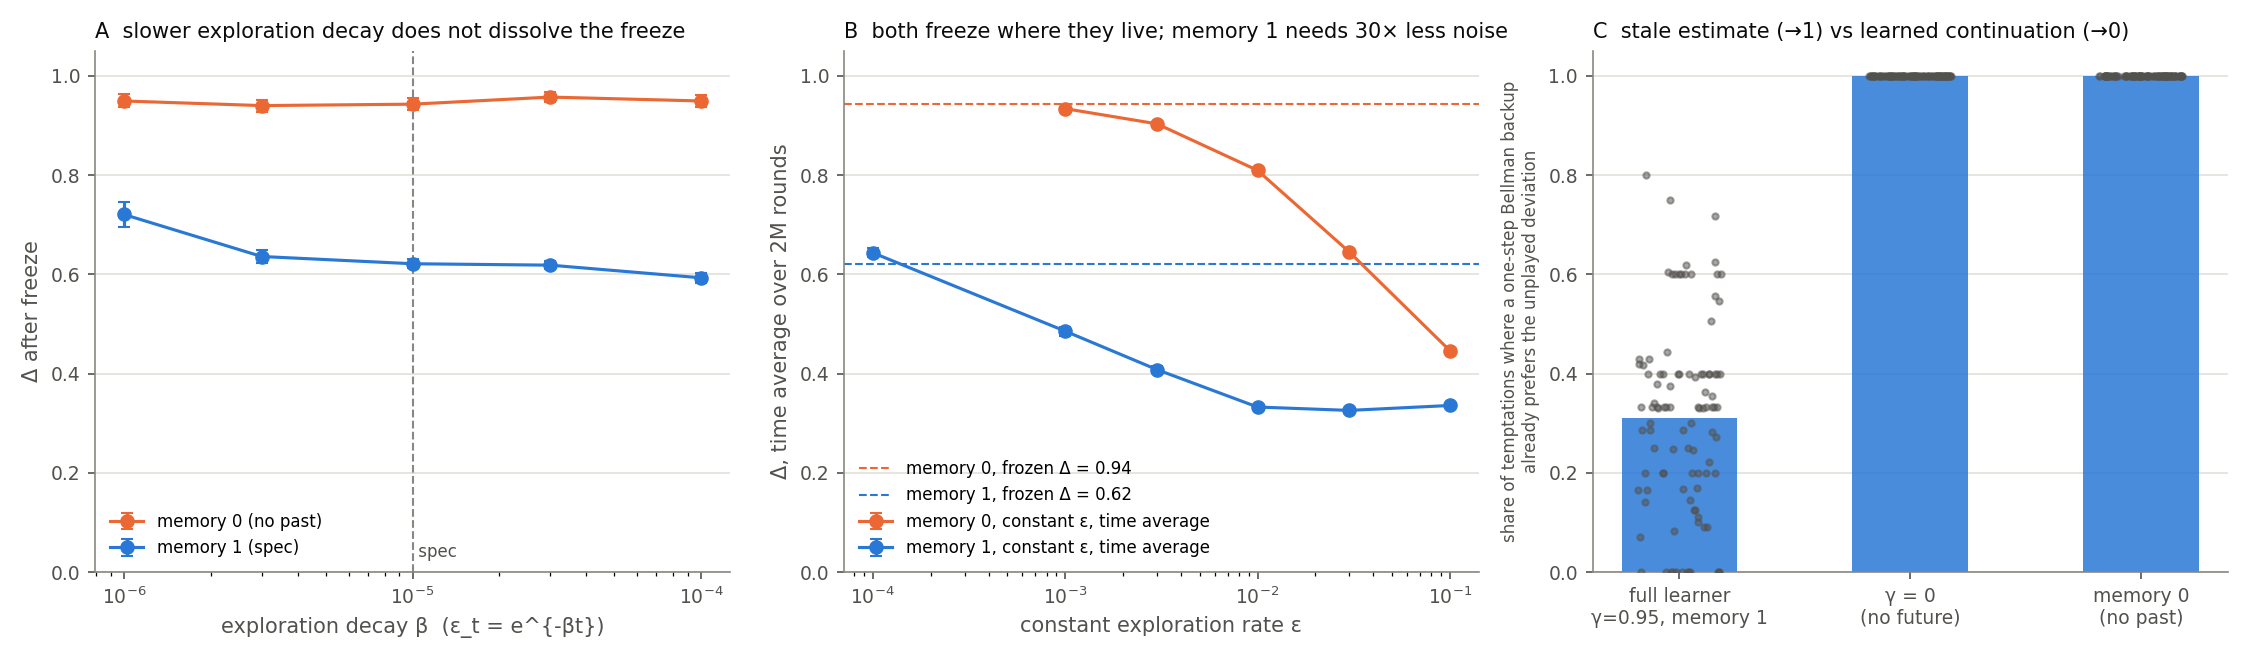
\includegraphics[width=\textwidth]{figures/phase1.png}
\caption{Three views of the Phase 1 evidence. Panel A: frozen $\Dl$ against the decay rate $\beta$ (Table~\ref{tab:sweep}); memory-0 is flat, memory-1 rises as decay slows. Panel B: time-average $\Dl$ under constant $\varepsilon$ (Table~\ref{tab:occupation}) with each learner's frozen value as a dashed line; both curves meet their frozen value as $\varepsilon \to 0$, memory-1 only at $\varepsilon = 10^{-4}$. Panel C: the share of temptations at which one Bellman backup already prefers the unplayed deviation (Table~\ref{tab:residual}), bar = mean, dots = seeds; the full learner sits at 0.31 with no seed at 1, the other two at 1 in every seed.}
\label{fig:phase1}
\end{figure}

Table~\ref{tab:occupation} and Panel B of Figure~\ref{fig:phase1} confirm the prediction for memory-0. The time average rises monotonically as $\varepsilon$ falls and reaches 0.934 at $\varepsilon = 0.001$, within 0.01 of the frozen 0.943; it is already within 5\% at $\varepsilon = 0.003$. The frozen price is the small-noise limit of where the exploring process spends its time. The block-to-block moves are large for memory-0, about \eur{28} in either direction at $\varepsilon \leq 0.03$ (Appendix~\ref{app:extra}), which is consistent with a process that jumps between the top and the bottom of the grid; the block average does not resolve the step-by-step walk down that the argument below assumes, so the asymmetry itself is not observed. 

We read this as a cycle of the Edgeworth type \citep{maskin1988}; what follows is a verbal argument that the experiments are consistent with, not a result, and Section~\ref{sec:discussion} states its limits. An undercut is discovered by an exploratory draw; the firm that is undercut sells less (60 to 40 MW if it was lowest, 20 to 0 if it was one of the tied high bidders), learns this, and undercuts back; the price falls by a rung whenever the second-lowest bid falls. Near the bottom a firm earning nothing loses nothing by raising its bid, and because the price is the second-lowest bid it takes one raise if a rival is already high and two if not; either way each step up is free, whereas each step down needs a specific exploratory draw at a specific time. If so, the exploring process should spend more time near the top the less noise there is, and freezing would sample that distribution; Table~\ref{tab:occupation} is consistent with this and does not test the chain itself. This is a statement about a learning dynamic on a discrete grid, not about strategy. The closest analogy is stochastic stability \citep{kandori1993,young1993}: as the noise vanishes, the states selected are those that take the most rare draws to leave and the fewest to reach, and here the high-price profiles are where the process is found. It is not the folk theorem \citep{fudenberg1986}: there is no threat, and with one state there is no memory to carry one.

The memory-1 learner also meets its frozen value, but far less easily. Its exploring process lives at $\Dl$ between 0.326 and 0.486 for $\varepsilon$ from 0.1 down to 0.001, below its frozen 0.621, and 0\% of blocks exceed \eur{55} for $\varepsilon \geq 0.03$. At $\varepsilon = 0.001$ it is still 0.14 below the frozen value. Only at $\varepsilon = 10^{-4}$, in a 30M-round run, does the time average reach 0.643 and meet it. Memory-0 is within 5\% of its frozen price at $\varepsilon = 0.003$; memory-1 needs roughly 30 times less noise for the same closeness. That is consistent with a coordinated cycle: three agents alternating between a high and a low profile, which any single random draw breaks for a stretch, and which re-forms only when draws are rare. The occupation measure separates the two learners by noise tolerance, not by kind. The Bellman-residual share of Section~\ref{sec:residual} remains the qualitative separator, and Panel C of Figure~\ref{fig:phase1} shows why: the memory-0 and $\gamma = 0$ seeds stack at 1, the full learner's seeds spread below it and none reaches 1. One caveat belongs here. The memory-1 curve has a single point at $\varepsilon = 10^{-4}$, so the location of its transition is not pinned down.

Three things change in the verdict of Section~\ref{sec:results}. The memory-0 price now has a candidate explanation. The experiments are consistent with its being the small-noise limit of an Edgeworth-type cycle run by $\varepsilon$-greedy learners on a discrete grid (a verbal argument, Section~\ref{sec:discussion}); it survives ten-fold slower decay, a restart of exploration from $\varepsilon_0 = 0.5$ that reassigns the low-bidder role in about 70\% of seeds, and a change of auction rule; and on this evidence it is a property of the learning dynamic, not evidence of collusion. The full learner does something the memory-0 learner does not: its deviation estimates are equally stale, but in 69\% of temptations the continuation it has learned is poor enough that a fresh estimate would not change the decision, and under constant exploration its time-average price sits far below its frozen value at noise levels ($\varepsilon \leq 0.003$) at which the memory-0 average is already within 5\% of its own frozen value. The $\Dl$-based ablation was right to fail, because price levels cannot tell these two learners apart, and the one measurement that can, the Bellman-residual share, needs the Q-table.

\section{Discussion}\label{sec:discussion}

Table~\ref{tab:indicators-summary} sets the four tests of Sections~\ref{sec:results} and~\ref{sec:phase1} side by side. Each row asks the same question: does the test tell a learner that has learned a continuation from one that carries a stale estimate, or does it merely record that the memory-1 learner can condition on rivals' bids and the memory-0 learner cannot?

\begin{table}[t]
\caption{What each indicator detects, and whether it separates the two learners. Notes: memory-1 column is the long (5M-round) run, 100 seeds; memory-0 column is the long memory-0 control, 100 seeds; ``discriminates'' asks whether the test tells learned continuation from a stale estimate, not merely whether the two columns differ.}
\label{tab:indicators-summary}
\centering
\footnotesize
\setlength{\tabcolsep}{4pt}
\begin{tabular}{p{1.6cm} p{3.2cm} p{3.6cm} p{3.0cm} p{2.9cm}}
\toprule
Test & Meant to detect & Memory-1 result & Memory-0 control & Discriminates? \\
\midrule
M3 punishment & Rivals answer a deviation, then forgive & Rivals react in 91\% of seeds (deviator firm 1); punish-forgive 21\%, no recovery 70\%, no reaction 9\% & No reaction in 100\% of seeds & No: it detects memory, which a one-state table lacks by construction \\
M4 ablation & Price needs memory and foresight & $\Dl = 0.621$; $\gamma = 0$ gives $0.370$, memory 0 gives $0.943$; neither below the $0.25$ threshold & Is the ablation & No \\
M5 temptation & Profitable deviation left unplayed & 100\% of seeds; mean gap $\eur{2{,}226}$ per round & 100\% of seeds; mean gap $\eur{1{,}448}$ per round & No: fires for the memory-0 control \\
Bellman residual & One fresh update would flip the decision & 31\% of temptations; 12 seeds at 0\%, none at 100\% & 100\% of temptations in every seed & Yes: 0.31 versus 1.00, no overlap across seeds \\
\bottomrule
\end{tabular}
\end{table}

\paragraph{A reading of the memory-0 price.}
What follows is a verbal argument, not a theorem; the evidence for it is the occupation measure of Section~\ref{sec:occupation} and the robustness results of Sections~\ref{sec:beta}, \ref{sec:reinject} and~\ref{sec:payasbid}. Because the clearing price is the second-lowest bid (Section~\ref{sec:market}), a lone undercut from a profile whose two lowest bids are tied sells 60 MW at the rivals' price and leaves the price where it was; at the all-cap profile that is a gain of $\eur{2{,}400}$ per round. This is why the M5 gap is large at every supra-competitive profile, and why the deviation round in M3 is profitable for the deviator; whether the deviation pays over the following rounds depends on the rivals' reaction and is not what M3 measures. The price falls only when a second firm follows the first down. On this reading a race to the bottom needs two firms to keep undercutting each other, and it stops wherever it stands when the exploratory draws that drive it become rare; the observed rest point, one firm at or near cost and two tied near the cap, is what such a stalled race looks like under this clearing rule. The walk down is a chain of learning events, each requiring a specific exploratory draw at a specific time; the move up from the bottom, where a firm has nothing to lose by raising its bid, needs a single event. Figure~\ref{fig:mechanism} draws the asymmetry. For the memory-0 learner the process spends its time near the top of the grid, more so the less exploration there is, and freezing the tables samples that distribution. The occupation measure in Section~\ref{sec:occupation} supports the last step of this argument, though not the asymmetry itself: the memory-0 time average rises from $\Dl = 0.446$ at $\varepsilon = 0.1$ to $0.934$ at $\varepsilon = 0.001$, within $0.01$ of the frozen $0.943$. The analogy is stochastic stability \citep{kandori1993,young1993}: as noise vanishes such a process selects the states that take the most rare draws to leave and the fewest to reach. We have computed no escape probabilities, so this is an analogy rather than a result, but the high-price profiles are where the memory-0 process is found. On this reading the memory-0 process is an Edgeworth-type cycle run by a learning rule \citep{maskin1988} rather than an instance of the folk theorem \citep{fudenberg1986}: with one state there is no memory to carry a threat. The memory-1 learner's frozen value is also the small-noise limit of its occupation measure, but a far more fragile one: its exploring process sits below that value until $\varepsilon = 10^{-4}$, roughly 30 times less noise than memory-0 needs, which is consistent with a coordinated cycle that single random draws break. The occupation measure separates the two learners by noise tolerance, not by kind (Section~\ref{sec:occupation}).

\begin{figure}[t]
\centering
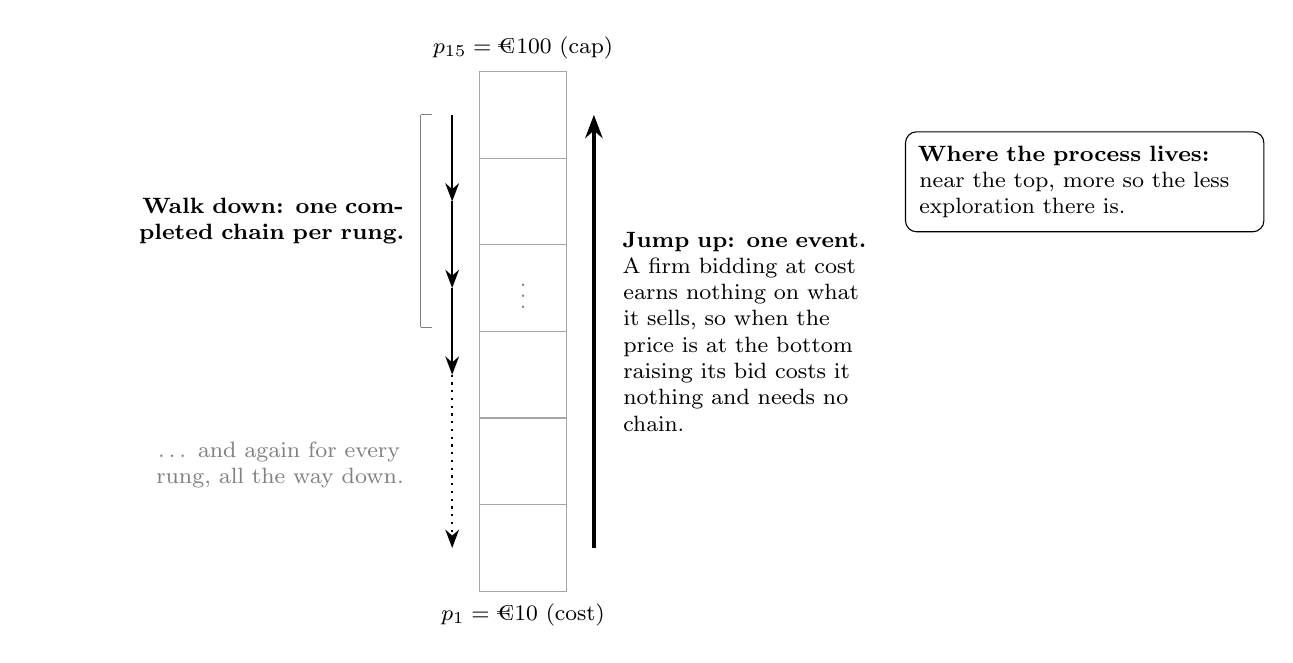
\begin{tikzpicture}[>=Stealth, font=\footnotesize, x=1cm, y=1cm]
% the bid ladder: six rungs stand for the fifteen
\foreach \i in {0,...,5} {\draw[gray!70] (0,\i*1.1) rectangle ++(1.1,1.1);}
\node[above=1pt] at (0.55,6.6) {$p_{15}=\eur{100}$ (cap)};
\node[below=1pt] at (0.55,0) {$p_{1}=\eur{10}$ (cost)};
\node[gray] at (0.55,3.85) {$\vdots$};
% left: the walk down, one completed chain per rung
\foreach \i in {5,4,3} {\draw[->, thick] (-0.35,\i*1.1+0.55) -- (-0.35,\i*1.1-0.55);}
\draw[->, thick, dotted] (-0.35,2.75) -- (-0.35,0.55);
\draw[gray] (-0.75,6.05) -- (-0.75,3.35);
\draw[gray] (-0.75,6.05) -- (-0.6,6.05);  \draw[gray] (-0.75,3.35) -- (-0.6,3.35);
\node[anchor=east, text width=4.6cm, align=right] at (-0.9,4.7)
  {\textbf{Walk down: one completed chain per rung.}};
\node[anchor=east, text width=4.6cm, align=right, gray] at (-0.9,1.6)
  {\ldots\ and again for every rung, all the way down.};
% right: the jump up, one event
\draw[->, very thick] (1.45,0.55) -- (1.45,6.05);
\node[anchor=west, text width=3.2cm, align=left] at (1.7,3.3)
  {\textbf{Jump up: one event.}\\ A firm bidding at cost earns nothing on what it sells, so when the price is at the bottom raising its bid costs it nothing and needs no chain.};
% the consequence
\node[draw, rounded corners, text width=4.2cm, align=left, inner sep=5pt, anchor=west] at (5.4,5.2)
  {\textbf{Where the process lives:} near the top, more so the less exploration there is.};
\end{tikzpicture}
\caption{A verbal reading of the memory-0 price (Section~\ref{sec:discussion}); it is not a theorem, and the asymmetry it draws was not measured directly. Rungs are the bid grid. On the left, each step down the grid would need a completed chain of learning events, each link an exploratory draw at the right moment. On the right, a firm at the bottom would raise its bid in one event, having nothing to lose. If the asymmetry holds it would concentrate the exploring process near the top; what Section~\ref{sec:occupation} does measure is that the process is found there, and that freezing samples that distribution.}
\label{fig:mechanism}
\end{figure}

\paragraph{What the indicators can and cannot do.}
The three behavioural tests were designed for a learner whose high price rests on anticipated retaliation. Here they cannot tell such a learner from one whose price is a property of the learning rule. M5 fires in 100\% of seeds for both learners: the memory-0 control leaves the same kind of money on the table, so the fingerprint does not require a learner that can anticipate anything. M4 fails because removing memory raises the price to $0.943$ rather than lowering it, and removing foresight leaves $0.370$, above the collapse threshold of $0.25$. M3 does separate the two, but for a trivial reason: a one-state table has nothing to react to, so it records no reaction in 100\% of memory-0 seeds. It confirms that the memory-1 learner's greedy policy varies with rivals' last bids, which its state definition permits but does not guarantee, and its verdict for a given seed changes with the identity of the deviator in 61 of 100 seeds. The residual is different in kind. It asks whether one fresh update of the deviation's value would flip the decision. For the memory-0 learner the answer is yes at every temptation in every seed. For the memory-1 learner it is yes at 31\% of temptations, no seed reaches 100\%, and twelve seeds sit at 0\%. In the remaining 69\% of memory-1 temptations the continuation after deviating, valued by the learner's own table, is low enough that a single fresh backup would leave the decision unchanged. That is a learned continuation, the thing tacit collusion consists of, measured on the table rather than inferred from behaviour. Whether a learned continuation of this kind deserves the name is a question this paper does not settle, and the measurement has a limit of its own: the continuation value it uses comes from the same table and may itself be stale (Section~\ref{sec:residual}).

Two consequences follow for anyone screening simulated bidding algorithms. First, in this market a high $\Dl$ together with a large unclaimed temptation does not by itself distinguish a learner that anticipates retaliation from one that cannot: the memory-0 control produces both. Whether the same holds in other non-pivotal auctions was not tested. Second, the residual needs the Q-table. It is a simulation-side diagnostic, available to a researcher, or to a firm auditing its own algorithm if that algorithm keeps a value table. None of this is a screen for real bid data, where only bids, prices and quantities are observed and no table exists to be read.

\paragraph{Relation to the literature.}
\citet{abada2023} and \citet{abada2024} reach a similar broad conclusion in a different market: outcomes that look collusive can arise from how independent learners explore. This paper agrees for the memory-0 learner and adds that the memory-1 learner is only partly of that kind. The mechanism detail here is different. Their concern is that learners fail to find the competitive outcome; here the freeze is not specific to the uniform-price rule, since it survives the change to pay-as-bid (Section~\ref{sec:payasbid}), though under uniform pricing the rule shapes where the process stops: at the (low, high, high) rest point the low bidder is paid the high price for its full 60 MW and has no profitable deviation, while each high bidder could earn \eur{1{,}543} more per round by shaving one rung (Section~\ref{sec:market}) but can discover that only through an exploratory draw. \citet{asker2022} find that the learning protocol, in particular what the algorithm is told about profits it did not earn, determines whether prices end high or low in their game. The memory-0/memory-1 contrast is a difference of state space rather than of updating rule, so it is not the protocol difference they study; what the two papers share is that a design choice inside the learner, not the incentives of the game, moves the outcome. The residual share separated the two learners' tables in this market; whether it would separate other protocol differences was not tested. \citet{banchio2022} find that the auction format decides whether Q-learning bidders settle at collusive-looking bids: below value under first-price rules, not under second-price rules. In this market the format moved the rest point but did not remove the freeze: under pay-as-bid the memory-0 $\Dl$ falls from $0.943$ to $0.845$, the most common frozen profiles change from one low bidder with two tied high bidders to symmetric ties, and every seed still converges with $\Dl$ above $0.5$.

\paragraph{Limits.}
The study is a simulation of one stylised single-node market with symmetric firms, inelastic and constant demand, no network or congestion, no multi-segment bid curves, and tabular learners only, so nothing is said about function-approximation learners. Apart from $\beta$ and the horizon the hyperparameters were not swept; $\alpha$, $\gamma$ and the grid come from the pre-registered specification. The punishment verdict uses fixed 12-round windows and a half-rung threshold; the nine long-run seeds with 5- or 7-cycles can be misread by those windows. The Bellman residual is a one-step backup with the current table, so $\max_{a'} Q_i(s', a')$ may itself be stale; a $k$-step rollout under the greedy policy would be stricter and was not done. The memory-1 occupation curve has one point at $\varepsilon = 10^{-4}$, so the transition is not located precisely. There is no theory: the Edgeworth-cycle argument is verbal. Finally, the two extra one-shot Nash equilibria on the grid ($\Dl = 0.07$ and $0.14$) mean the competitive benchmark is a band $[0, 0.14]$ rather than a point; all reported $\Dl$ lie far above it.

\paragraph{Next steps.}
A $k$-step rollout residual would remove the dependence on possibly stale continuation values; whether the separation survives it is an open question. A run at an exploration rate between $\varepsilon = 10^{-3}$ and $10^{-4}$ would locate where the memory-1 occupation measure meets its frozen value. A two-firm, three-price version of the market might be solvable by hand and might turn the verbal cycle argument into a statement about basins of the noisy dynamic. Network constraints and multi-segment bids are separate future work: they change the pivotality on which the argument above rests and should be studied on their own.

\section{Conclusion}\label{sec:conclusion}

Three independent tabular Q-learners bidding into a stylised uniform-price electricity auction settle at prices far above marginal cost. With one round of memory the collusion index reaches $\Dl = 0.62$ after five million rounds; without memory it reaches $\Dl = 0.94$. That much is an observed fact. The question the paper set out to answer is whether the standard evidence would let one call these outcomes tacit collusion. In this market it does not.

The three behavioural indicators borrowed from the literature do not discriminate. The punishment test finds reactions to a forced undercut in the memory-1 runs and none in the memory-0 runs, which is what it should find, but its verdict for a given seed changes with the identity of the firm made to deviate. The shortsightedness ablation fails its own pre-registered collapse criterion for both ablations: removing the discount factor lowers the price but leaves it well above cost, and removing memory raises it. The temptation test finds a profitable unplayed deviation in every seed of the full learner and of the memoryless control, and in 95\% of $\gamma = 0$ seeds, the rest sitting at one-shot Nash profiles. An indicator that fires on a control which cannot, by construction, condition on rivals is not measuring anticipated retaliation.

One test does separate the two learners. A single Bellman backup on the best unplayed deviation would reverse the decision in 100\% of temptations for the memoryless learner and in 31\% for the learner with memory. In the remaining memory-1 temptations the continuation value after deviating, taken from the learner's own table, is low enough that a fresh estimate would not change the decision, which is what a learned continuation is. Deviation estimates are stale in every configuration, the full learner included; what differs is the consequence. For the memory-0 learner we offer a reading rather than a theorem: its price is consistent with the small-noise limit of an Edgeworth-type cycle on a coarse grid, and with one state there is no threat to carry. That price is not an accident of the exploration schedule, since it survives ten-fold slower decay and a restart at $\varepsilon_0 = 0.5$ that reassigns the low-bidder role in 70\% of seeds.

The result cuts in two directions. Supra-competitive prices from independent learners are easy to produce and robust to the perturbations we tried, so they deserve attention. But the evidence usually offered for calling them collusion cannot bear that weight here, and the one test that separates a learned continuation from a stale estimate, without settling whether the former deserves the name, requires the Q-table. It is a simulation-side tool, not a screen for real bid data; whether a data-side analogue exists is the open question this paper leaves.


\bibliographystyle{plainnat}
\bibliography{refs}

\appendix
\section{Reproduction}\label{app:repro}

Everything in this paper is produced by the Python package \texttt{collusim} (version 0.1.0; numpy and numba are its only runtime dependencies) and three scripts that sit on top of it. The repository is at \url{https://github.com/pradeep221b/algorithmic-collusion-auction}. To reproduce every table and figure, clone the repository and run, in order,
\begin{verbatim}
pip install -e ".[figures,test]"
pytest
python experiments.py
python indicators.py
python phase1.py <sweep|reinject|residual|payasbid|occupation|
                  occupation_mem1|occupation_mem1_long|fig>
\end{verbatim}
\texttt{pytest} runs the 31 tests (clearing rule, Q-update, indicators on hand-built policies, package surface). \texttt{experiments.py} runs the price-level study of Section~\ref{sec:results} and the ablations of Table~\ref{tab:m4}. \texttt{indicators.py} runs the punishment, ablation and temptation verdicts. \texttt{phase1.py} takes one subcommand per experiment of Section~\ref{sec:phase1}; \texttt{occupation} is the memory-0 occupation run, \texttt{occupation\_mem1} the memory-1 run at the same five noise levels, \texttt{occupation\_mem1\_long} the single 30M-round point at $\varepsilon = 10^{-4}$, and \texttt{fig} draws Figure~\ref{fig:phase1} from the stored results.

The training loop is compiled with numba and runs at about 0.4 s per million rounds per seed. Measured at 100 seeds, one process per job, on a 12-thread laptop with no GPU: the six base configurations take about 9 minutes in total; the ten cells of the $\beta$ sweep about 27 minutes; the two pay-as-bid runs about 4 minutes; the re-injection runs about 6 minutes; the Bellman residual about 2 minutes; the indicator battery on all six configurations about 3 minutes; each occupation curve about 10 minutes and the single 30M-round point about 20 minutes. Run sequentially the whole study takes about two hours; with the jobs overlapped, under an hour and a half. The environment used was Python 3.14 with numpy 2.x.

Every number in the paper is stored per seed, in the \texttt{results} directory. The file \texttt{<config>.json} holds, for each seed, the frozen-play $\Dl$, the convergence round and the last-round profile; the file \texttt{indicators\_\allowbreak<config>.json} holds every punishment, ablation and temptation verdict; the file \texttt{phase1\_\allowbreak<name>.json} holds the Phase-1 results. The final Q-tables are saved as \texttt{.npz} files next to the JSON summaries and are not committed to the repository; the re-injection and residual experiments read them, so those two subcommands need the base runs to have been executed first. The re-injection restarts draw from a separate seed stream, so the new exploration draws are independent of the original training draws.

One naming convention differs between the code and the paper. The code indexes firms 0, 1, 2; the paper calls them firms 1, 2, 3 throughout. Firm 1 in the paper is agent 0 in the code, and the ``deviator = firm 1'' rows of Section~\ref{sec:results} are the code's default \texttt{deviator=0}.

\section{Parameters and procedures}\label{app:params}

\paragraph{Price grid.} The 15 admissible bids are the points of \texttt{linspace(10, 100, 15)}, so rung $r$ has price $p_r = 10 + (r-1)\cdot 90/14$ \texteuro/MWh and one rung is \eur{6.43}. Table~\ref{tab:app-grid} lists them. In the body of the paper bid profiles are written with prices rounded to the nearest euro, so that (10,\,16,\,16) means rungs 1, 2, 2.

\begin{table}[htbp]
\centering
\caption{The bid grid. Notes: prices in \texteuro/MWh; the marginal cost is \eur{10} and the price cap \eur{100}.}
\label{tab:app-grid}
\begin{tabular}{rr@{\qquad}rr@{\qquad}rr}
\toprule
$r$ & $p_r$ & $r$ & $p_r$ & $r$ & $p_r$ \\
\midrule
1 & 10.00 & 6 & 42.14 & 11 & 74.29 \\
2 & 16.43 & 7 & 48.57 & 12 & 80.71 \\
3 & 22.86 & 8 & 55.00 & 13 & 87.14 \\
4 & 29.29 & 9 & 61.43 & 14 & 93.57 \\
5 & 35.71 & 10 & 67.86 & 15 & 100.00 \\
\bottomrule
\end{tabular}
\end{table}

\paragraph{Learner parameters.} Learning rate $\alpha = 0.15$, discount $\gamma = 0.95$ (or 0 in the ablation), exploration $\varepsilon_t = e^{-\beta t}$ with $\beta = 10^{-5}$, so that $\varepsilon = 0.37$ at $10^5$ rounds, $0.05$ at $3\times 10^5$ and $4.5\times 10^{-5}$ at $10^6$. With memory 1 the state is last round's full bid profile, $15^3 = 3{,}375$ states; with memory 0 there is one state. The table is initialised at $Q_0[s,a] = \mathbb{E}[\text{profit}(a,\ \text{rivals uniform})]/(1-\gamma)$. Horizons are 1M and 5M rounds and every run goes to the full horizon. These values were fixed in the specification before any result was seen and were never tuned.

\paragraph{Convergence.} A run is recorded as converged when no agent's greedy action, in any state, changed during the last 100,000 rounds. The flag is recorded and reported; it never stops a run.

\paragraph{Frozen play and $\Dl$.} Learning and exploration are switched off, the agents play greedily from the final state for 1,000 rounds, the first 100 rounds are dropped, and $\Dl = (\bar p - 10)/90$ is computed from the mean clearing price $\bar p$ of the remaining 900.

\paragraph{Punishment procedure.} Learning stays frozen. Greedy play first settles for 200 warm-up rounds. Six pre-deviation rounds are recorded. In the next round the deviator is forced to bid \eur{10}; the rivals play their greedy actions. Twenty-four post-deviation rounds of greedy play follow. A counterfactual path is generated from the same state with no forced bid. The verdict is read off the rivals' bids relative to the counterfactual in two windows, rounds 1--12 and 13--24 after the deviation, with a threshold of half a rung, $\eur{3.21}$: \emph{punish--forgive} if the rivals' mean bid is at least \eur{3.21} below the counterfactual in rounds 1--12 and back within \eur{3.21} in rounds 13--24; \emph{punish, no recovery} if below in both windows; \emph{no reaction} if the rivals do not move. A case is a \emph{no-op} when the deviator was already bidding \eur{10}, so that the forced bid changes nothing. Twelve-round windows were chosen because 12 is divisible by the cycle lengths 1 to 4 and 6; periods 5 and 7 are not covered, which affects 9 seeds in the long run.

\paragraph{Temptation.} At every state on the converged cycle and for every firm, the best one-shot deviation profit, with rivals held at their greedy actions, minus the realised profit. A seed has ``unclaimed temptation'' if any such gap is positive.

\paragraph{Bellman residual.} For every temptation on the converged cycle, indexed by firm $i$, state $s$, played action $a_i$ and best unplayed deviation $a_{\mathrm{dev}}$, let $a_{-i}(s)$ denote the rivals' greedy actions at $s$ and $s'(a)$ the state that follows when firm $i$ plays $a$ against them. Define the one-step target and residual of an action $a$ as
\begin{align*}
\mathrm{target}_i(s,a) &= \pi_i\big(a,\ a_{-i}(s)\big) + \gamma \max_{a'} Q_i\big(s'(a),\ a'\big), \\
\mathrm{resid}_i(s,a) &= \mathrm{target}_i(s,a) - Q_i(s,a),
\end{align*}
evaluated with the current, frozen table. The residual on the played action is a check: it must be near zero on a converged cycle, and it is. The residual on $a_{\mathrm{dev}}$ measures how far the stored deviation value is from what one fresh update would make it. A backup \emph{prefers the deviation} when $\mathrm{target}_i(s,a_{\mathrm{dev}}) > Q_i(s,a_i)$, that is, when a single update of the deviation entry would already flip the greedy choice. The share reported in Table~\ref{tab:residual} is the fraction of a seed's temptations at which this holds, averaged over seeds. Its limitation is that $Q_i(s'(a),\cdot)$ is itself taken from the same table and may be stale; a $k$-step rollout would be stricter and was not done.

\section{Additional results}\label{app:extra}

\paragraph{Punishment by deviator.} Table~\ref{tab:m3} reports the long-run verdicts with firm 1 as the forced deviator. Table~\ref{tab:app-deviator} repeats the split for firms 2 and 3. The shares are similar in aggregate, but the verdict for a given seed changes with the identity of the deviator in 61 of 100 seeds. In 47\% of seeds at least one of the three deviators produces a punish--forgive verdict.

\begin{table}[htbp]
\centering
\caption{Punishment verdicts in the long run (5M rounds, memory 1, 100 seeds) by identity of the forced deviator. Notes: percentages of seeds; the firm-1 row is the one in Table~\ref{tab:m3}; 2\% of firm-1 cases are no-ops (the deviator was already at \eur{10}).}
\label{tab:app-deviator}
\begin{tabular}{lrrr}
\toprule
Deviator & punish--forgive & punish, no recovery & no reaction \\
\midrule
Firm 1 & 21 & 70 & 9 \\
Firm 2 & 20 & 69 & 11 \\
Firm 3 & 17 & 73 & 10 \\
\bottomrule
\end{tabular}
\end{table}

\paragraph{Mean paths around the deviation.} Table~\ref{tab:app-path} gives the mean clearing price and the rivals' mean bid gap to the counterfactual in the two post-deviation windows, for all 100 long-run seeds and for the two main verdict subsets. Averaged over all seeds the rivals' bids sit 16.7 below the counterfactual in rounds 1--12 and 13.5 below in rounds 13--24, and the clearing price falls from \eur{66.0} before the deviation to \eur{45.1} and then \eur{49.4}, against a counterfactual of \eur{65.9} in both windows. The forgive subset falls to \eur{49.9} in the first window and returns almost exactly to its counterfactual in the second (gap 0.2, price \eur{63.2} against \eur{65.4}); the no-recovery subset stays about 20 below it and its price remains in the low forties.

\begin{table}[htbp]
\centering
\caption{Mean price paths around a forced one-round undercut, long run (5M rounds, memory 1, deviator firm 1). Notes: ``rivals' cut'' is how far the rivals' mean bid sits below its counterfactual value, in \texteuro/MWh; prices are mean clearing prices in \texteuro/MWh; the counterfactual is the same rounds with no forced bid.}
\label{tab:app-path}
\footnotesize
\setlength{\tabcolsep}{4pt}
\begin{tabular}{lrrrrrr}
\toprule
 & & \multicolumn{2}{c}{rivals' cut} & \multicolumn{3}{c}{clearing price} \\
\cmidrule(lr){3-4}\cmidrule(lr){5-7}
Seeds & $n$ & rounds 1--12 & rounds 13--24 & rounds 1--12 & rounds 13--24 & counterfactual \\
\midrule
All & 100 & 16.7 & 13.5 & 45.1 & 49.4 & 65.9 \\
Punish--forgive & 21 & 10.9 & 0.2 & 49.9 & 63.2 & 65.4 \\
Punish, no recovery & 70 & 20.5 & 19.1 & 41.8 & 43.8 & 66.2 \\
\bottomrule
\end{tabular}
\end{table}

\paragraph{Converged profiles.} Table~\ref{tab:app-profiles} lists the most common last-round bid profiles on frozen play for the $\gamma = 0$ long run and the two pay-as-bid runs. The $\gamma = 0$ learner ends on long irregular cycles: only 20 of 100 seeds have period 4 or less and periods run up to 25, and its most common profiles are one-shot Nash profiles or near them, with one firm at cost and two tied one or more rungs above. The pay-as-bid runs end at symmetric ties, each firm selling a third of demand at its own bid, at a higher level without memory than with it.

\begin{table}[htbp]
\centering
\caption{Most common last-round bid profiles on frozen play, 5M rounds, 100 seeds per run. Notes: bids rounded to the nearest euro; count is the number of seeds ending at that profile; permutations of an asymmetric profile are pooled.}
\label{tab:app-profiles}
\begin{tabular}{llr}
\toprule
Run & Profile & Seeds \\
\midrule
$\gamma = 0$, memory 1 & (10, 16, 16) & 15 \\
 & (10, 36, 36) & 10 \\
 & (10, 42, 42) & 10 \\
 & (10, 29, 29) & 9 \\
 & (16, 42, 42) & 7 \\
 & (10, 55, 55) & 7 \\
\midrule
Pay-as-bid, memory 0 & (68, 68, 68) & 16 \\
 & (94, 94, 94) & 12 \\
 & (81, 81, 81) & 9 \\
 & (87, 87, 87) & 8 \\
\midrule
Pay-as-bid, memory 1 & (55, 55, 55) & 13 \\
 & (49, 49, 55) & 9 \\
 & (61, 61, 61) & 8 \\
 & (49, 49, 49) & 8 \\
\bottomrule
\end{tabular}
\end{table}

\paragraph{Block-to-block moves in the occupation runs.} In the constant-$\varepsilon$ runs of Table~\ref{tab:occupation} the price is averaged in blocks, and a move is counted when the block mean changes by more than \eur{5}. The two learners move differently. The memory-0 learner makes large jumps: about \eur{28} in either direction at $\varepsilon \le 0.03$ and about \eur{22} at $\varepsilon = 0.1$, which is the signature of the walk down the grid and the single jump back up described in Section~\ref{sec:discussion}. The memory-1 learner makes small ones: about \eur{10} at $\varepsilon \le 0.003$, about \eur{8} at $\varepsilon = 0.01$, about \eur{4}--\eur{5} at $\varepsilon = 0.03$, and none at all at $\varepsilon = 0.1$, where its time-average $\Dl$ is 0.336 and no block exceeds $\eur{55}$.


\end{document}
